\documentclass[hidelinks,a4paper,12pt]{tesiinfo}

%%Pacchetti utili anche se non necessari
\usepackage{amsfonts}

\usepackage{amsmath}

\usepackage{latexsym}


\usepackage{tabularx}
%% Supporto alla lingua italiana, dipende dal vostro ambiente latex
\usepackage[italian]{babel}
%% Supporto per i caratteri accentati
\usepackage[utf8]{inputenc}
%% Supporto alle figure
\usepackage{graphicx}
%% Supporto alle figure wrappate nel testo
\usepackage{wrapfig}
%% Supporto alle didascalie
\usepackage{caption}
%% Supporto alle figure composte
\usepackage{subfigure}
%% Supporto alle didascalie per figure composte
%%\usepackage{subcaption}
%% Supporto ai link esterni (URL)
\usepackage[bookmarks=true]{hyperref}

%% Supporto alla creazione di colonne multiple nel documento
\usepackage{multicol}
%% Supporto al comando \cite per BibTex
\usepackage{cite}
%% Supporto per i listati di codice
\usepackage{listings}
%% Supporto allo stile per il codice PHP creato da Nicola Sacco e Daniele Di Pompeo
\usepackage{listings,xcolor}
\usepackage{caption}

\definecolor{mygreen}{rgb}{0,0.6,0}
\definecolor{mygray}{rgb}{0.5,0.5,0.5}
\definecolor{mymauve}{rgb}{0.58,0,0.82}

\lstset{ %
  backgroundcolor=\color{white},   % choose the background color; you must add \usepackage{color} or \usepackage{xcolor}
  basicstyle= \scriptsize\ttfamily,% the size of the fonts that are used for the code
  breakatwhitespace=false,         % sets if automatic breaks should only happen at whitespace
  breaklines=true,                 % sets automatic line breaking
  commentstyle=\color{mygreen},    % comment style
  deletekeywords={...},            % if you want to delete keywords from the given language
  escapeinside={\%*}{*)},          % if you want to add LaTeX within your code
  extendedchars=true,              % lets you use non-ASCII characters; for 8-bits encodings only, does not work with UTF-8
%   frame=single,                    % adds a frame around the code
  keywordstyle=\color{red},       % keyword style
  language=php,                 % the language of the code
  morekeywords={*,new},            % if you want to add more keywords to the set
%   numbers=left,                    % where to put the line-numbers; possible values are (none, left, right)
%   numbersep=5pt,                   % how far the line-numbers are from the code
%   numberstyle=\tiny\color{mygray}, % the style that is used for the line-numbers
  rulecolor=\color{black},         % if not set, the frame-color may be changed on line-breaks within not-black text (e.g. comments (green here))
  showspaces=false,                % show spaces everywhere adding particular underscores; it overrides 'showstringspaces'
  showstringspaces=false,          % underline spaces within strings only
  showtabs=false,                  % show tabs within strings adding particular underscores
  stepnumber=2,                    % the step between two line-numbers. If it's 1, each line will be numbered
  stringstyle=\color{blue},     % string literal style
  tabsize=2,                       % sets default tabsize to 2 spaces
}

\DeclareCaptionFont{white}{\color{white}\tiny}
\DeclareCaptionFormat{listing}{\colorbox[cmyk]{0.43, 0.35, 0.35,0.01}{\parbox{\textwidth}{\hspace{15pt}#1#2#3}}}
\captionsetup[lstlisting]{format=listing,labelfont=white,textfont=white, singlelinecheck=false, margin=0pt, font={bf,footnotesize}}
%% Supporto al glossario
\usepackage[style=altlist, toc=true]{glossary} % can be obtained from http://www.ctan.org/tex-archive/macros/latex/contrib/glossary/
%% Richiesta di creazione del glossario
\makeglossary
%% Inclusione del file con i termini del glossario
\storeglosentry{Esempio}{name={Nome da visualizzare}, description={Descrizione nel glossario}}



\titolo{Realizzazione di un prototipo della versione Cloud SaaS della suite IBM BigFix: Automazione del deployment e del testing}
\laureando{Beniamino Negrini}
\relatore{Serafino Cicerone}
\annoaccademico{2016/2017}

%%Usare i seguenti comandi se si ha un correlatore:
\setcorrelatoreuno
\correlatoreuno{Dott. Marco Secchi}

%%Usare i seguenti comandi se si hanno due correlatori (NB: questi comandi sono alternativi a quelli precendenti):
%\setcorrelatoredue
%\correlatoreuno{Nome e cognome del primo correlatore}
%\correlatoredue{Nome e cognome del secondo correlatore}

%%Usare i seguenti comandi se si ha un relatore esterno (NB: questi comandi possono essere utilizzati con quelli precedenti):
\setesterno
\relatoreesterno{Dott. Bernardo Pastorelli}

%%Usare i seguenti comandi se si sta scrivendo una tesi di laurea specialistica
\setspecialistica

\begin{document}


\maketitle
   
  \begin{dedication}
  \textit{Dedica a piè pagina}
  \end{dedication}



\contentspage
 
  \chapter{Introduzione}

\paragraph{}
(prima bozza, verrà raffinata al termine della stesura dei capitoli)

\paragraph{}
E' sempre più evidente che il cloud computing è il futuro del software. La rivoluzione consta nella distribuzione dei servizi di calcolo e nella virtualizzazione delle risorse, dando così all'utente la sensazione di un utilizzo centralizzato. Tutto ciò si è reso realizzabile dal momento in cui l'accesso alla rete è divenuto possibile da sempre più dispositivi e con velocità di connessione sempre maggiore.
\paragraph{}
La tematica del cloud computing è stata centrale nel mio lavoro di tesi presso l'azienda IBM (International Business Machines Corporation) nella sua sede di Roma. Ho partecipato attivamente alla realizzazione di un prototipo software, ossia la versione SaaS della suite IBM BigFix. BigFix è una suite di prodotti dedicati alle aziende che risolvono problematiche di Endpoint Security e di compliance di dispositivi a determinate politiche aziendali. Tramite questi prodotti si ottiene pieno controllo su tutti i dispositivi aziendali. Si possono ad esempio rilevare eventuali attacchi o si possono distribuire aggiornamenti e patch.
\paragraph{}
La sfida da me raccolta è quindi proprio quella di portare tutto questo arsenale di strumenti nella leggerezza del cloud. Rendendolo disponibile, nel giro di pochi minuti, anche a chi è sempre stato intimorito dalla difficoltà di installazione di uno strumento così potente, ma allo stesso tempo complesso.
  \chapter{IBM BigFix}

\section{BigFix}
I prodotti della suite IBM BigFix consentono di monitorare e gestire in tempo reale un elevato numero di dispositivi connessi (fino a 250.000). Questi possono essere sia fisici che virtuali, come ad esempio server, desktop, notebook, dispositivi mobili, tablet, POS, ATM e chioschi self-service. Gli utenti principali di questi prodotti sono gli amministratori di sistema. Tramite le applicazioni BigFix possono avere il pieno controllo sugli endpoint. Possono ad esempio distribuire software, applicare delle patch, effettuare il deploy di sistemi operativi, proteggere da attacchi di rete e molto altro.
\begin{figure}[h!]
	\centering
	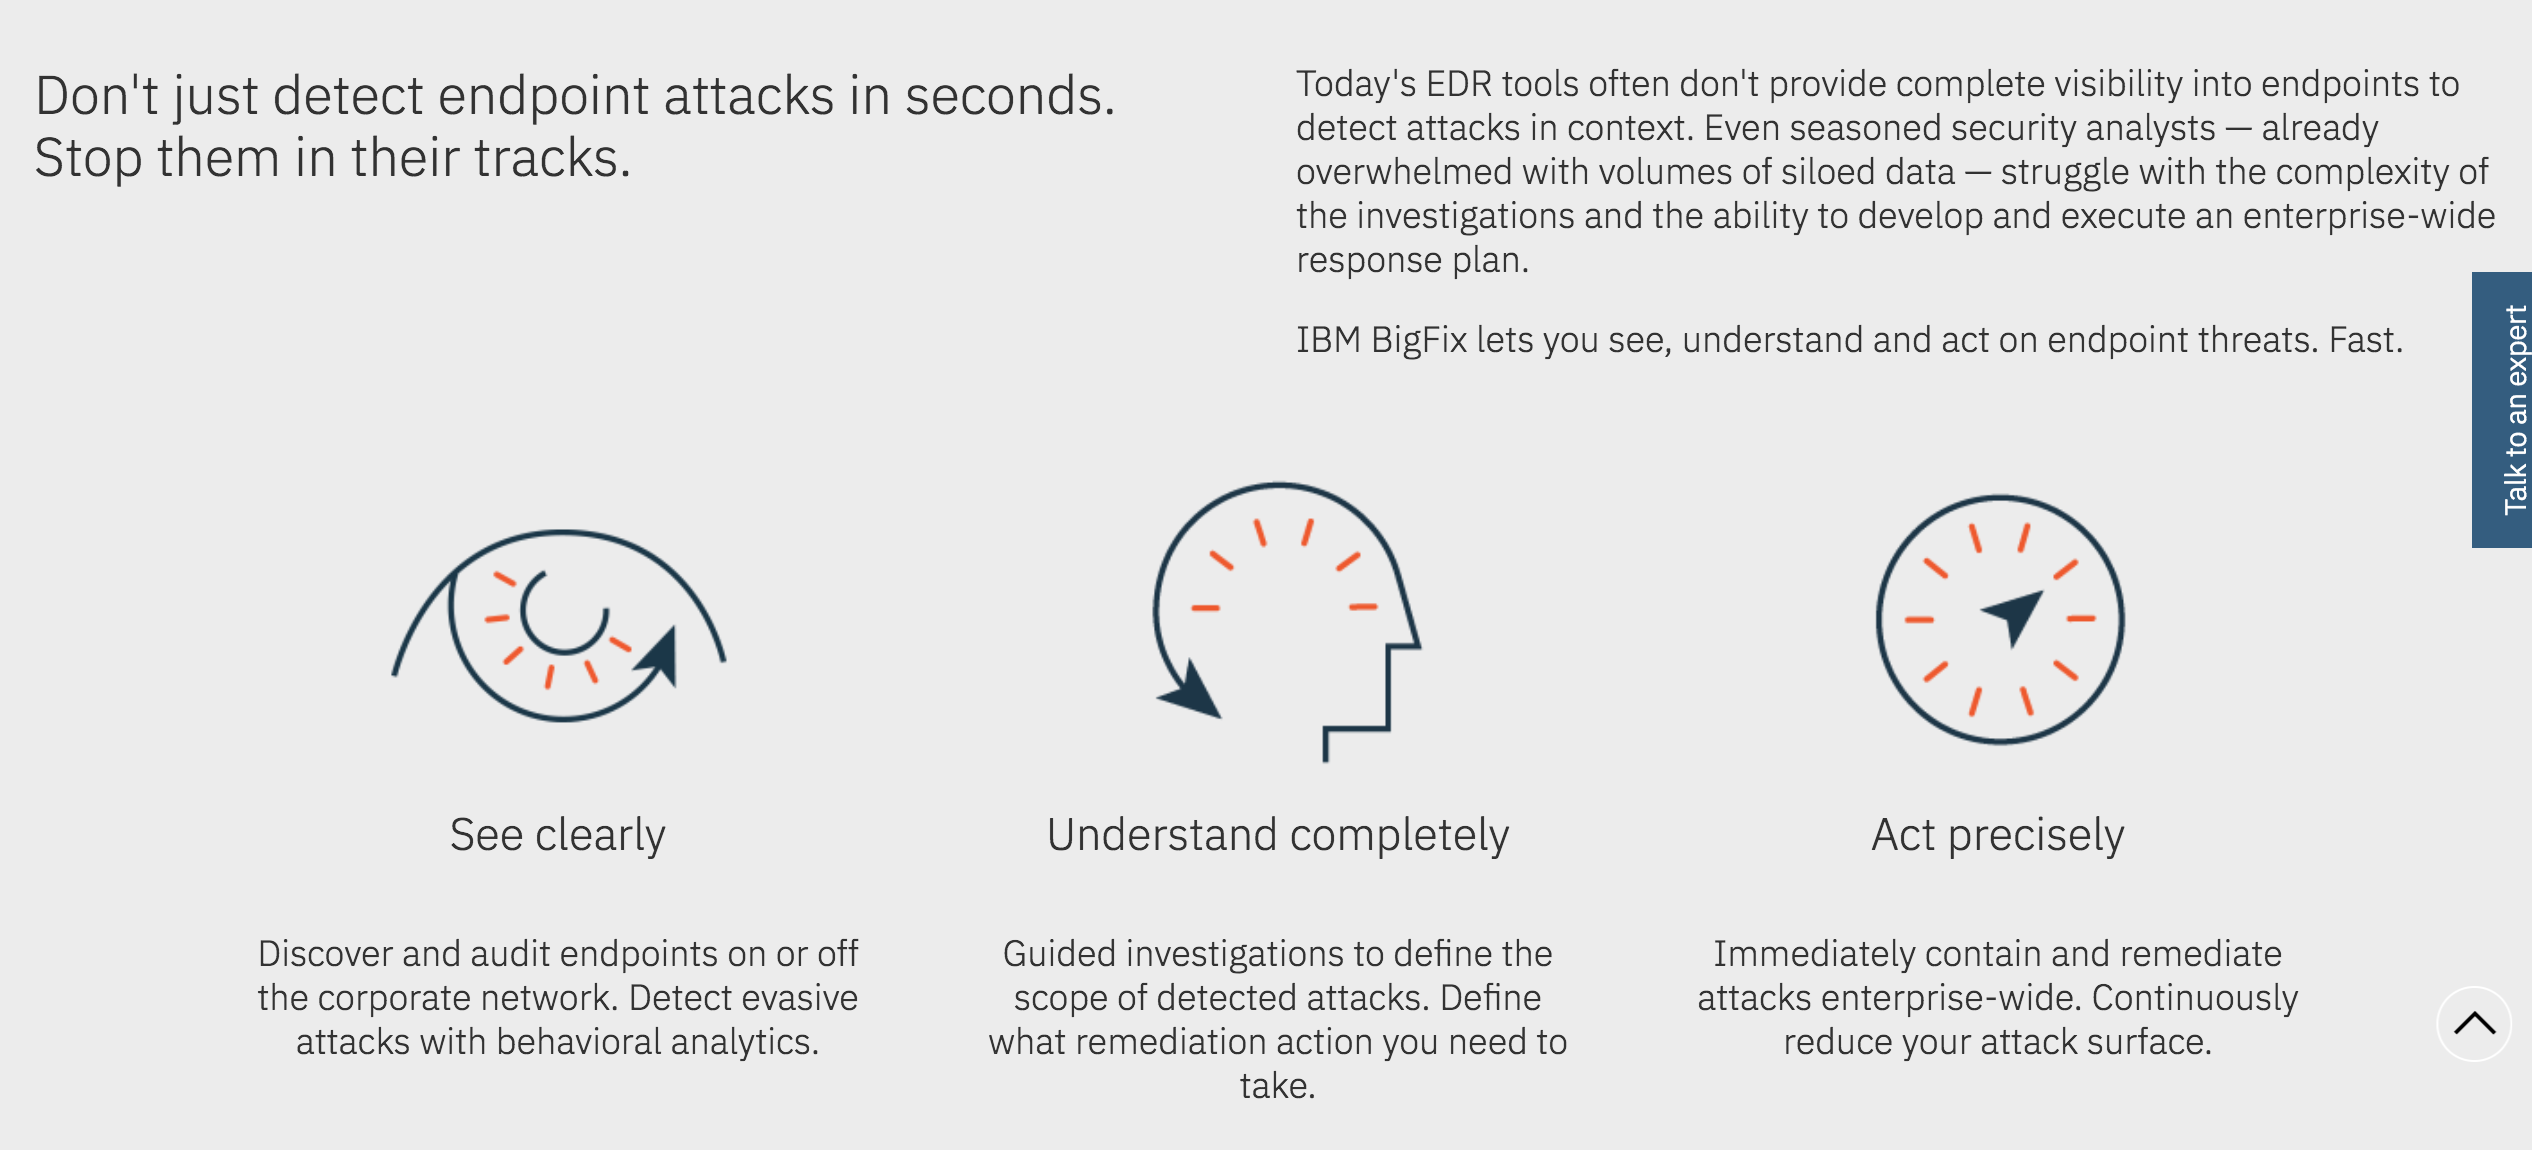
\includegraphics[width=\textwidth,keepaspectratio=true]{capitoli/imgs/BigFixManifest.png}
	\caption{Breve header descrittivo di BigFix dal sito web di IBM Security}
\end{figure}
\subsection{Architettura}
L'architettura di BigFix può essere, per sua natura, molto articolata, nel caso si debba gestire un numero elevato ed eterogeneo di dispositivi. Essa si basa sul consolidato pattern stilistico client/server, ma con una struttura leggermente variata, prevedendo l'inserimento di un ulteriore layer frapposto tra client e server, i Relay, i quali sono fondamentali per bilanciare il carico.
\paragraph{}
Ma partiamo subito con un esempio per avere un ponto di riferimento.
\begin{figure}[h!]
	\centering
	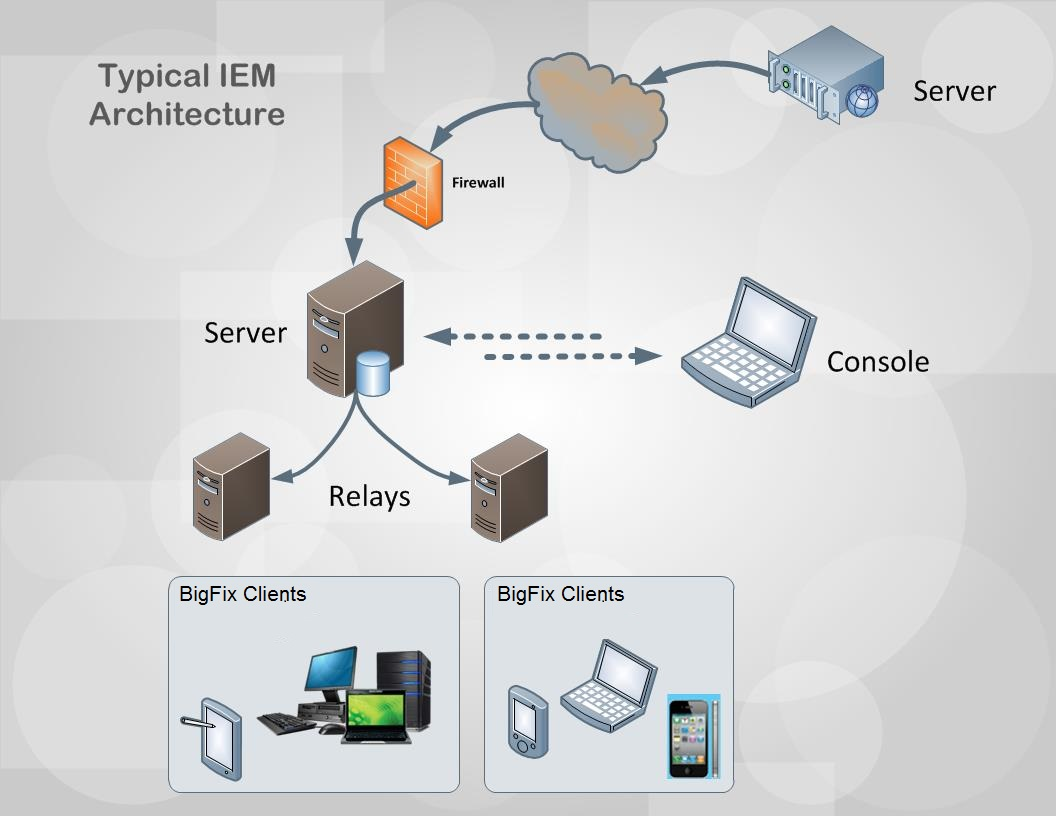
\includegraphics[width=\textwidth,keepaspectratio=true]{capitoli/imgs/IEMArchitecture.png}
	\caption{Un'architettura BigFix di esempio}
\end{figure}
Come possiamo notare, l'elemento centrale è il server di BigFix, il quale ha lo scopo di raccogliere dei particolari messaggi chiamati Fixlet. Questi messaggi dovono poi venire inoltrati ai Relay. E' competenza dei Relay interagire con i singoli client e assicurarsi l'esecuzione delle Fixlet. Le Fixlet, infatti, altro non sono che delle azioni che devono essere necessariamente compiute dai client. Una sorta di "catalogo" delle Fixlet più utili può essere trovato sul Content server che è accessibile via internet da gli utilizzatori di BigFix. In tutto ciò la finestra dalla quale opera l'amministratore è ovviamente la Console, la quale monitora tutto il flusso di lavoro di BigFix. Andiamo ora ad analizzare le singole componenti dell'architettura.
\paragraph{Servers}
Il server coordina tutto il flusso di informazioni e si preoccupa di salvare le informazioni sul database. Al tempo stesso però, lascia agli Agent il compito di effettuare analisi ed eseguire azioni specifiche. Ciò consente di liberare il server da un pesantissima computazione. Per questo motivo il server stesso può gestire un altissimo numero di client.
\paragraph{Relays}
I Relay si comportano come una cache tra i client e il server e sono di numero variabile in base al numero di client. Aiutano il server a gestire i dispositivi anche se funzionalmente non sono altro che client che sono stati promossi a Relay, aggiungendo a loro dei servizi. A questo punto i client non si interfacceranno mai con il server, alleggerendone così notevolmente il workload. Possono, ad esempio, più client richiedere un download al Relay, il quale effettuerà un'unica richiesta al server
\paragraph{Agents}
Un Agent è installato su ogni client facente parte dell'architettura di BigFix. Essi hanno il compito di raccogliere le Fixlet, tramite le quali sono in grado di compiere tutte le azioni necessarie. Un Agent fa dei continui check per confrontare lo stato del dispositivo con le policy stabilite. Appena scopre che il dispositivo è fuori dalla compliance, informa il server ed agisce subito per porre rimedio e, al termine dell'attività, l'Agent informa nuovamente il server sull'esito dell'operazione.
\paragraph{Web Reports}
I Web Reports costituiscono il componente che consente ad utenti autorizzati di monitorare tutti i dispositivi di BigFix. Si può, in questo modo, tenere traccia di vulnerabilità, azioni richieste e molto altro.
\paragraph{Consoles}
La Console permette agli amministratori di interagire con tutti i client dell'ambiente BigFix. Gli utenti possono così distribuire velocemente patch e configurazioni.
\paragraph{Content Server}
Il Content server è una sorta di repository. Contiene Fixlet a bassa personalizzazione che fanno fronte a esigenze più o meno comuni a tutti gli utenti BigFix. Possono essere prelevate ed utilizzati per i propri fini.
\paragraph{}
BigFix, da un punto di vista logico, si suddivide in due grandi macro-componenti, la Platform e le Applications. La prima svolge la funzione di layer sopra la quale vengono sviluppate tutte le funzionalità dello strato di applications. Questa organizzazione consente una chiara suddivisione delle competenze da parte di progettisti, sviluppatori, tester e assistenti dei clienti. Il team della Platform si concentra quindi nel fornire una solida infrastruttura al team delle Applications, il quale svilupperà i singoli strumenti al servizio dell'utente.
\subsection{BigFix Platform}
La Platform è una tecnologia multi-layer scritta in linguaggio C++ che agisce come colonna portante di tutta l'infrastruttura di BigFix. Essa svolge infatti funzioni fondamentali, spesso utilizzate anche da altre applicazioni dei layer superiori. Le attività della Platform sono fondamentali per la sussistenza dell'architettura che abbiamo descritto poco fa.

\subsection{BigFix Applications}
Tutti i prodotti applicativi che fanno parte di questo componente consentono di gestire in maniera semplice le operazioni inerenti alla security. A differenza della Platform, sono implementate in linguaggio Java o JavaScript ed hanno funzionalità atomiche tra di loro. Sono l'interfaccia principale con il quale interagisce l'amministratore aziendale.

\paragraph{BigFix Lifecycle}
Questa è l'applicazione che l'amministratore utilizza per gestire il ciclo di vita degli endpoint fisici. Ha una visibilità completa su di essi e pone rimedi immediati. Tra le funzioni principali ci sono quelle di power management, software distribution e OS deployment. 
\paragraph{BigFix Patch}
E' l'applicazione che consente la distribuzione di patch sia a livello di applicativi che a livello di sistema operativo.
\paragraph{BigFix Compliance}
Si utilizza questa applicazione per garantire la compliance dei dispositivi, identificare irregolarità e risolverle.
\paragraph{BigFix Protection}
Questa applicazione viene adoperata per garantire una protezione real-time contro qualsiasi genere di malware (virus, trojan, worms, spyware, rootkits e altre minacce web). Ha ovviamente effetto sia sugli endpoint fisici che sulle macchine virtuali.
\paragraph{BigFix Inventory}
Come dice la parola stessa, questa applicazione si occupa di analizzare gli endpoint e generare un inventario di tutti i software su essi installati, generando dei report ed evidenziando, eventualmente, le irregolarità.

\subsection{Fixlets}
Le Fixlet sono il metodo attraverso il quale si svolgono tutte le operazioni, come distribuzione di software, installazioni di patch e configurazioni. Esse sono dei messaggi inoltrati ai client di BigFix e utilizzano un linguaggio di query specifico, il Relevance.
\subsubsection{Il linguaggio Relevance}
Con una Fixlet si può anche ispezionare un desiderato aspetto di un client. A tale scopo viene adoperato il linguaggio Relevance. Esso, infatti, consente di interrogare il client, identificandone caratteristiche dell'hardware o del software tramite particolari costrutti, gli Inspectors. Una necessità può essere infatti quella di applicare una Fixlet solamente a dei client con determinate caratteristiche hardware/software oppure che si trovano in stati ben definiti. Si può, in questo modo, facilmente identificare il corretto sottoinsieme di client ai quali è destinata una nuova Fixlet ed applicarla solo ad essi.

\section{IBM}
Come detto, il lavoro di tesi si è svolto nell'ambito di un progetto formativo stipulato tra l'Università dell'Aquila e IBM Italia Spa. Questo progetto ha previsto un tirocinio svolto nella seda di Roma con obiettivo: "Esplorazione e prototipazione di metodi per portare prodotti BigFix su cloud", per l'appunto la realizzazione del prototipo di BigFix Saas. 
\paragraph{}
La storia dell'IBM ha inizio nei primi decenni del novecento, ma è dagli anni settanta che entra nel mercato dell'informatica, soprattutto nel settore hardware. Negli ultimi venti anni il business si è spostato sempre più sul software. In particolare soluzioni cognitive e piattaforme cloud.
\paragraph{IBM Security}
Presso la sede di Roma presente il più importante laboratorio IBM italiano, il Rome Software Lab. Nella divisione italiana ci si concentra prevalentemente sullo sviluppo back-end. Una grossa fetta del laboratorio fa parte della divisione Security di IBM. Il portfolio di Security contiene per l'appunto prodotti che si occupano di diversi aspetti della security aziendale, tra questi BigFix è uno dei più consolidati.

\section{SaaS Exploration Project}
Lo scopo del progetto al quale ho partecipato con il mio lavoro è quello di esplorare le tecnologie esistenti nel panorama cloud e realizzare il prototipo della versione SaaS di BigFix. A questo scopo, oltre a me, sono state allocate altre tre persone full time al conseguimento del progetto, sotto la guida dell'Architect Bernardo Pastorelli.

\subsection{Il framework SCRUM}
Il team adotta il framework agile SCRUM. Questo modo di operare è di sempre maggiore diffusione ed è basato su un approccio iterativo e incrementale nello sviluppo software. Il design e lo sviluppo sono divisi in iterazioni, denominate "Sprint", della durata fissa di due settimane. Queste due settimane terminano sempre con una versione funzionante del prodotto, il quale viene mostrato in una demo che evidenzia le nuove features implementate.
\paragraph{}
SCRUM utilizza un approccio empirico alla progettazione. La filosofia di fondo del framework è quella che la conoscenza deriva dall'esperienza, e quindi tutte le scelte che si prendono nel corso della progettazione devono avvenire alla luce di una sempre maggiore esperienza, la quale si ottiene avendo a disposizione il prima possibile un sottoinsieme del prodotto a se stante, testabile ed usabile. Dì qui l'approccio fortemente iterativo e incrementale massimizzando le opportunità di feedback. 
\paragraph{} 
All'inizio del progetto vengono definiti i requisiti del prodotto (item), i quali vengono da un'attenta analisi dei bisogni dell'utente. Ogni bisogno viene modellato con una Epica, che a sua volta viene prioritizzata e aggiunta al Product Backlog che le indicizza. Le Epiche vengono poi scomposte in User Stories, le quali si suddividono a loro volta in Task, ossia l'elemento atomico del progetto la cui implementazione viene presa in carico da un singolo componente del team.
\paragraph{}
L'inizio di uno Sprint è sempre caratterizzato da un meeting in cui si pianificano gli obiettivi. In questo contesto si fa sempre riferimento al Backlog incentrandosi sulle User Stories ancora non coperte. Si cerca quindi di suddividersi i Task in modo tale da avere a fine Sprint quelle nuove funzionalità usabili e dimostrabili. Demo che viene svolta sempre con la presenza di tutto il team e anche di colleghi di altri laboratori IBM.
\subsection{Sistemi di controllo di versione}
Da un'organizzazione di questo tipo ne scaturisce la necessità di tool di controllo di versione che permettano una fluida gestione del codice e della programmazione in parallelo tra i diversi componenti del team.
\paragraph{GitLab}
A tal scopo si è adottato ormai da tempo, da tutto il team di BigFix, il software di controllo di gestione distribuito Git e una repository aziendale che consiste in una versione enterprise ad hoc per IBM di GitLab, un hosting service molto simile a GitHub. 
\begin{figure}[h!]
	\centering
	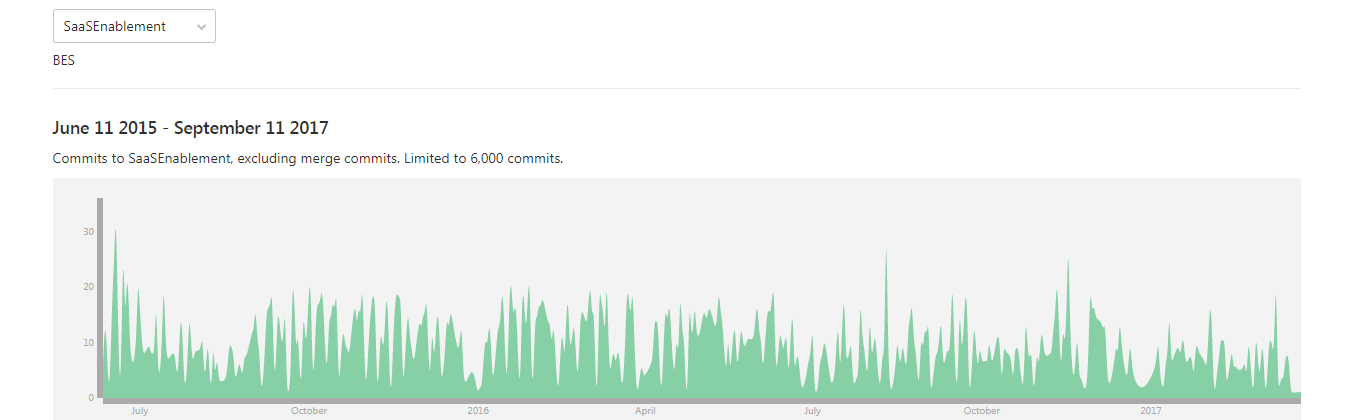
\includegraphics[width=\textwidth,keepaspectratio=true]{capitoli/imgs/GitLabGraph.PNG}
	\caption{Panoramica degli ultimi contributi nel branch del progetto SaaS}
\end{figure}
\paragraph{}
Il flusso di lavoro è il seguente. Quando inizia il proprio task, il componente del team si pone su un proprio branch personale sul quale effettua i propri commit. Al termine del task viene fatta una merge request sul branch principale, solo una volta che si è testato il codice, per aggiungere i propri contributi al progetto. A questo punto, dopo una review effettuata da componenti del team accreditati, il nuovo branch verrà mergiato con il branch principale.
\subsection{RTC}
E' ovviamente necessario un tool che coordini anche la suddivisione dei task all'interno del team. A tal fine abbiamo utilizzato un software di IBM, ovvero Rational Team Concert (RTC), il quale è disponibile anche esternamente e gratuito nel caso di piccoli team. Esso offre comodi strumenti di agile planning e gestione di ciclo di vita del software. Ogni componente del team può così tracciare facilmente le aree di sua competenza. E' possibile inoltre usufruire di tool per il source control, controllo dei difetti e gestione delle build.
\begin{figure}[h!]
	\centering
	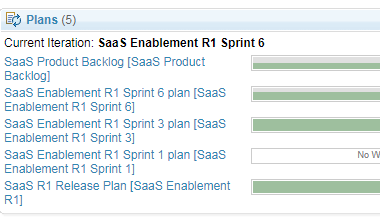
\includegraphics[width=0.5\textwidth,keepaspectratio=true]{capitoli/imgs/rtc2.PNG}
	\caption{RTC. Un'esempio di come viene monitorato il completamento dei diversi sprint}
\end{figure}



  \chapter{Il Cloud e le sue sfaccettature}

\section{Cloud Computing}
La differenza tra il possedere e l'utilizzare. E' questo l'aspetto cruciale del cambiamento apportato dal cloud computing rispetto al software tradizionale. Le risorse, che siano quelle di archiviazione, elaborazione o altro, non sono mai ad hoc per un singolo utilizzatore, ma vengono assegnate on demand e appartengono ad un insieme condiviso da tutti gli altri utenti del prodotto. Attraverso internet ogni utente può accedere a queste risorse in qualsiasi momento. Tali risorse vengono opportunamente allocate in maniera dinamica e completamente automatizzata. Si possono utilizzare così anche software non installati sul proprio computer o usufruire di una memoria di massa accessibile da qualsiasi dispositivo.
\paragraph{}
L'esperienza utente che si vuole fornire però è quella di un utilizzo esclusivo della risorsa, come nei software tradizionali. In realtà la risorsa viene solo sapientemente distribuita tra tutti coloro che la richiedono. Ciò fa si che, potenzialmente, un singolo utente possa acquisire risorse notevolmente maggiori rispetto ai software che utilizzano la macchina locale.
\begin{figure}
	\centering
	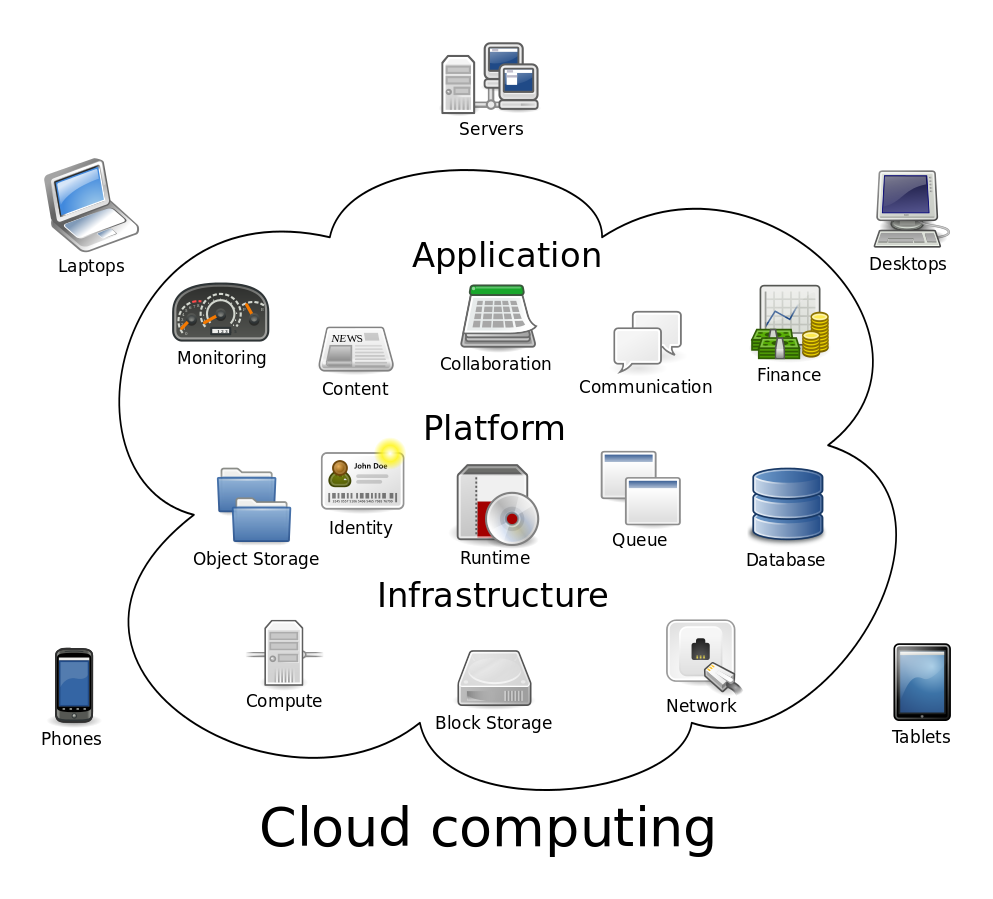
\includegraphics[width=0.5\linewidth]{capitoli/imgs/CloudComputing}
	\caption{Diagramma logico di una rete Cloud Computing}
	\label{fig:cloudcomputing}
\end{figure}
\subsection{Vantaggi del Cloud Computing}
\begin{itemize}
	\item Costo: \\
	Con l'avvento del cloud tutta la gestione dell'infrastruttura sottostante al software diviene a carico del provider. Vengono eliminate spese per la gestione dei data center locali. Facendo riferimento alla versione SaaS di BigFix ad esempio, il cliente viene sollevato dal pesante onere di utilizzare server locali e gestirne le relative connessioni. Il provider ospita tutto l'hardware di cui il cliente ha bisogno.
	
	\item Velocità: \\
	Anche qui ci risulta molto utile prendere come esempio la suite di BigFix. Quando un nuovo cliente acquista il prodotto nella sua versione on-premises, un'incaricato di IBM si reca presso il cliente e lì inizia un processo di installazione della suite che può impiegare diverse ore. Nello scenario SaaS il cambiamento è radicale. E' sufficiente che il cliente compili una form online, dopo alcuni minuti poi riceve una mail con il link per accedere al servizio.
	
	\item Prestazioni \\
	Una delle motivazioni principali per la quale si sceglie di fare uso del clud computing sono proprio le prestazioni, soprattutto se si adotta il paradigma PaaS. Richiedendo tramite cloud le risorse di calcolo, si può fare affidamento a dei provider che fanno dei server ad alte prestazioni il loro punto di forza. L'utente può, in questo modo, abbattere dei bottleneck che altrimenti risulterebbero di grande impedimento. Nel 2016 IBM mette per la prima volta a disposizione pubblicamente un computer quantistico, proprio attraverso una piattaforma cloud (IBM Q). Questo può rappresentare un esempio estremo in ottica prestazioni, ma che può rendere un'idea di quale potrà essere il trend nei prossimi anni.
	
	\item Affidabilità \\
	Operazioni di mirroring da parte dei provider dei servizi cloud fa sì che il backup dei dati sia continuo ed economico. Molto spesso i provider hanno data center sparsi in molte parti del mondo, ciò aumenta la resistenza a guasti o addirittura catastrofi che possono verificarsi. Ovviamente questo grado di replicazione dei servizi è impensabile nella fruizione on premise dei prodotti.
\end{itemize}

\section{Tipologie di servizi Cloud}
Il termine Cloud risulta essere in realtà molto generico. Esso comprende diverse tipologie di fornitura dei servizi, a seconda della risorsa che viene offerta dal provider. La maggior parte dei servizi di Cloud Computing rientrano in tre tipologie principali: Infrastruttura distribuita come Servizio (IaaS, Infrastructure as a Service), Piattaforma distribuita come Servizio (PaaS, Platform as a Service) e Software come un Servizio (SaaS, Software as a Service). Oltre a queste tipologie, annoveriamo anche altre soluzioni come il DaaS (Data a a Service) e l'HaaS (Hardware as a Service). Andiamo a vedere nel dettaglio come, a seconda della modalità di utilizzo del paradigma Cloud, queste strategie si differenziano. 
\begin{figure}
	\centering
	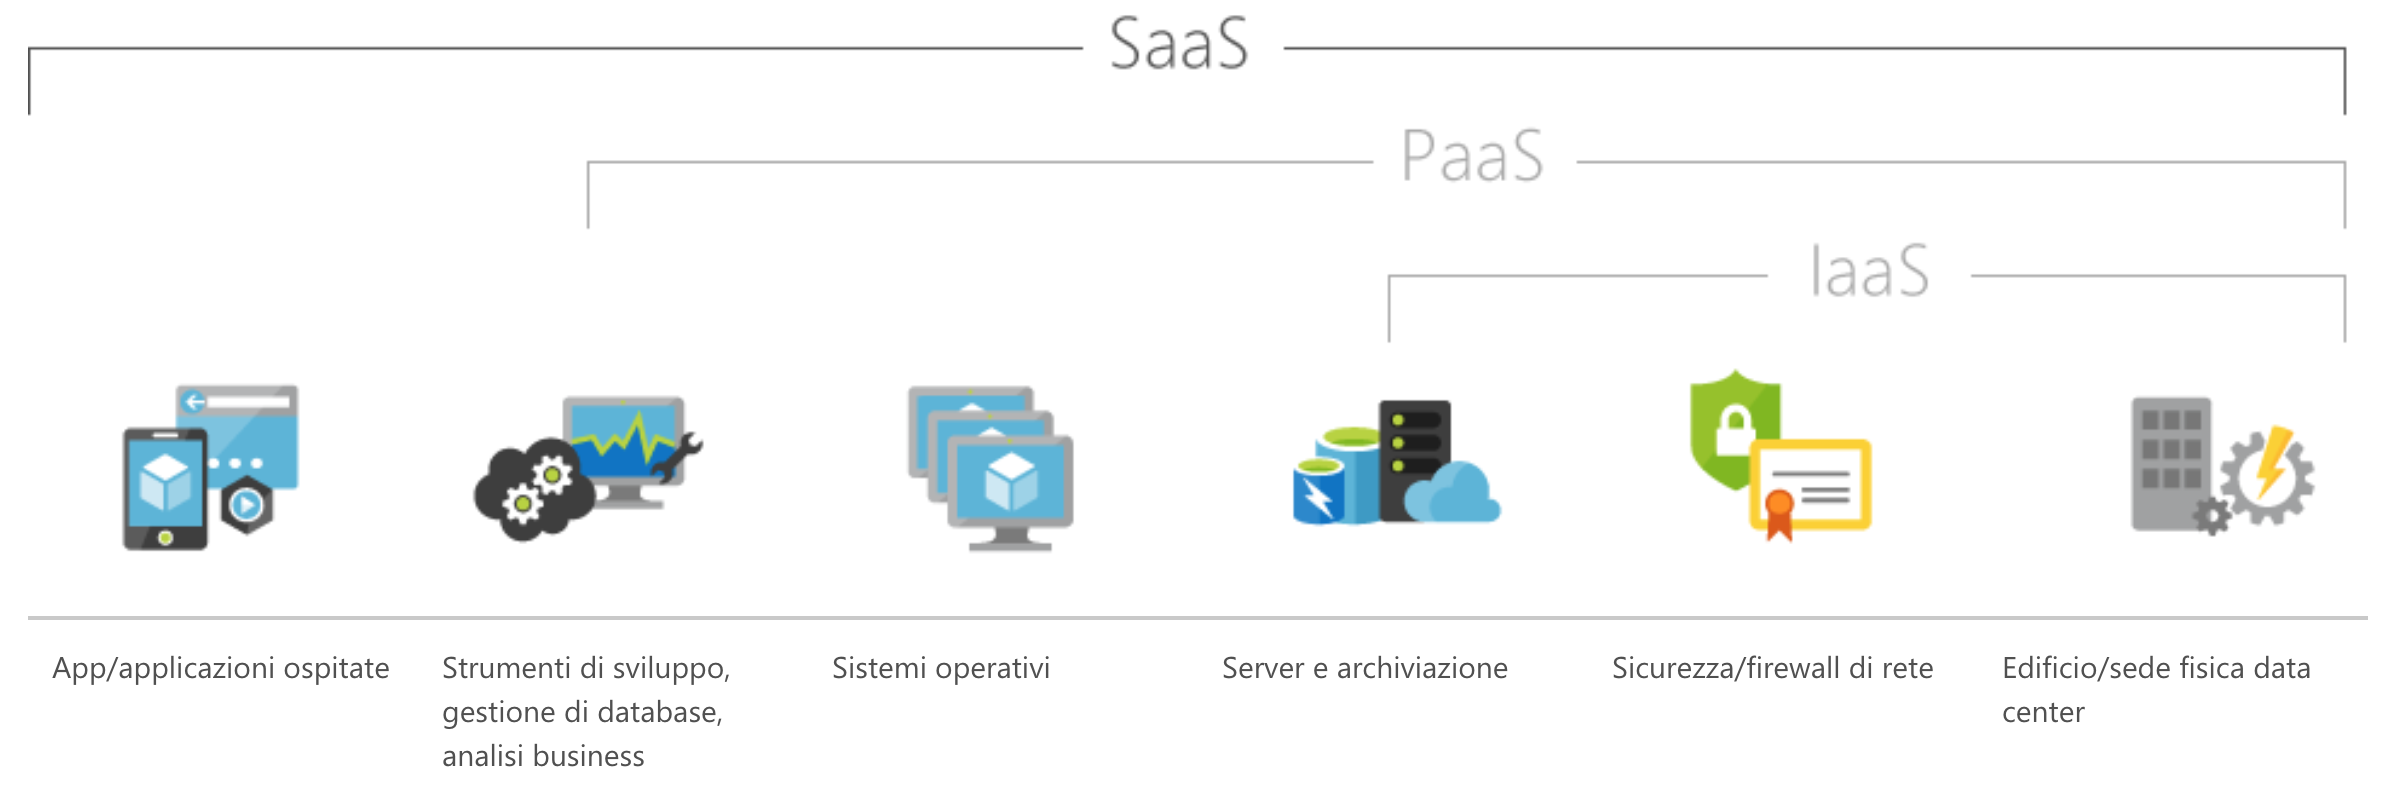
\includegraphics[width=0.7\linewidth]{capitoli/imgs/TipologieCloud}
	\caption{Panoramica delle principali tipologie Cloud}
	\label{fig:tipologiecloud}
\end{figure}

\subsection{IaaS, Infrastructure as a Service}
E' la tipologia più basilare. Vengono messe a disposizione piattaforme di elaborazione. Utilizzando un IaaS si affittano le infrastrutture utili ai propri scopi, come ad esempio server, macchine virtuali (VMs), risorse di archiviazione, reti e sistemi operativi. Può, inoltre, essere messo a disposizione anche hardware in remoto. Il provider di servizi cloud gestisce l'infrastruttura, mentre l'utente acquista, installa, configura e gestisce il software, tra cui sistemi operativi, middleware e applicazioni.
\paragraph{Vantaggi}
Una soluzione IaaS è quella che garantisce maggiore flessibilità. Tra i vantaggi principali ricordiamo:
\begin{itemize}
	\item  Elevata scalabilità \\
	Il modello IaaS permette una scalabilità verticale rapida ed economica
	\item Rapidità di innovazione \\
	Nel caso del lancio di un nuovo prodotto basato sulla piattaforma IaaS, il tempo di attesa per le nuove configurazioni infrastrutturali è solamente dell'ordine di pochi minuti.
	\item Adattabilità alle richieste \\
	Un modello IaaS è estremamente flessibile alle variazioni delle richieste. Si possono facilmente aumentare le risorse nei momenti di picco e ridurle quando non è necessario, risparmiando quindi denaro.
	
\end{itemize}
\subsection{PaaS, Platform as a Service}
Una piattaforma distribuita come servizio (PaaS, Platform as a Service) è un ambiente cloud di sviluppo completo. Una soluzione PaaS è progettata per consentire il ciclo completo dello sviluppo delle applicazioni: creazione, test, distribuzione, gestione e aggiornamento. L'utente ha tutta la libertà di sviluppare gli applicativi a proprio piacimento, ma lavora con componenti software già pronti all'utilizzo (i microservices). Questi componenti non sono localizzati presso chi utilizza il cloud, bensì presso il provider, il quale si occupa del loro mantenimento e aggiornamento. Il modello PaaS consente di evitare le spese e la complessità legate all'acquisto e alla gestione di licenze software, middleware e infrastruttura delle applicazioni sottostanti o strumenti di sviluppo. L'utente gestisce le applicazioni e i servizi che sviluppa e il provider cloud si occupa di tutto il resto.
\paragraph{Vantaggi}
Uno scenario PaaS riduce quindi notevolmente la quantità di codice da scrivere semplificando quindi il lavoro dello sviluppatore e aumentandone la produttività. Inoltre risulta molto più semplice così il porting di un prodotto da web a mobile e viceversa. Componenti molto complessi e costosi possono essere messi a disposizione, con un utilizzo limitato, anche per sviluppatori che altrimenti non potrebbero permetterselo. 
\subsubsection{IBM Bluemix}
Troviamo, sempre all'interno di IBM, uno dei principali servizi cloud PaaS presenti sul mercato: IBM BlueMix. L'utente può usufruire di un'astrazione di molte componenti utili allo sviluppo. Si può, ad esempio, fare uso di Database specifici, di moduli dedicati all'IoT, di tecnologie Blockchain e molto altro. Ne vediamo alcuni esempi nella figura 3.3
\begin{figure}[h!]
	\centering
	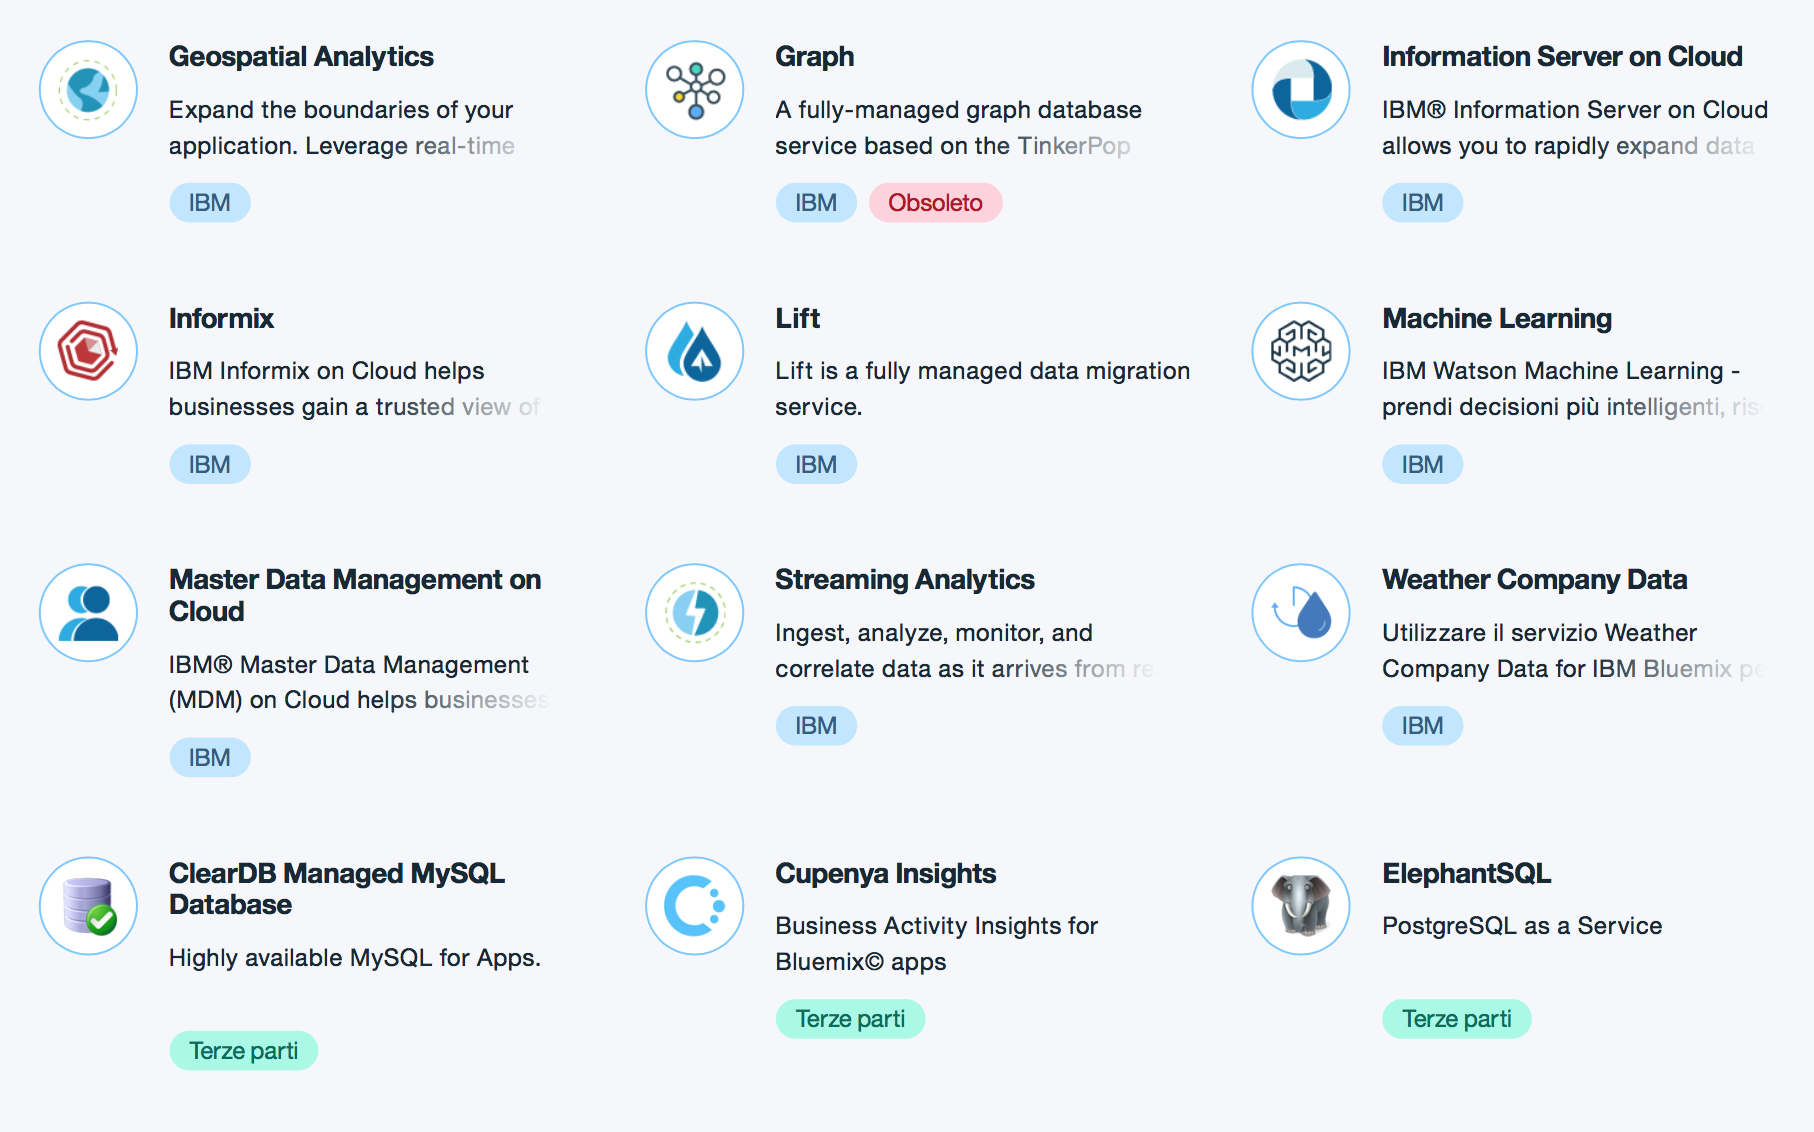
\includegraphics[width=\textwidth,keepaspectratio=true]{capitoli/imgs/catalog.png}
	\caption{Esempi di moduli presenti nel catalogo BlueMix}
\end{figure}
\subsubsection{IBM Watson}
Tra le componenti sviluppate da IBM merita una menzione anche Watson. Watson è un sistema di intelligenza artificiale in grado di rispondere a domande espresse in un linguaggio naturale. Tra le funzionalità ci sono quelle di elaborazione del linguaggio naturale, information retrieval, rappresentazione della conoscenza, ragionamento automatico e tecnologie di apprendimento automatico.
\begin{figure}[h!]
	\centering
	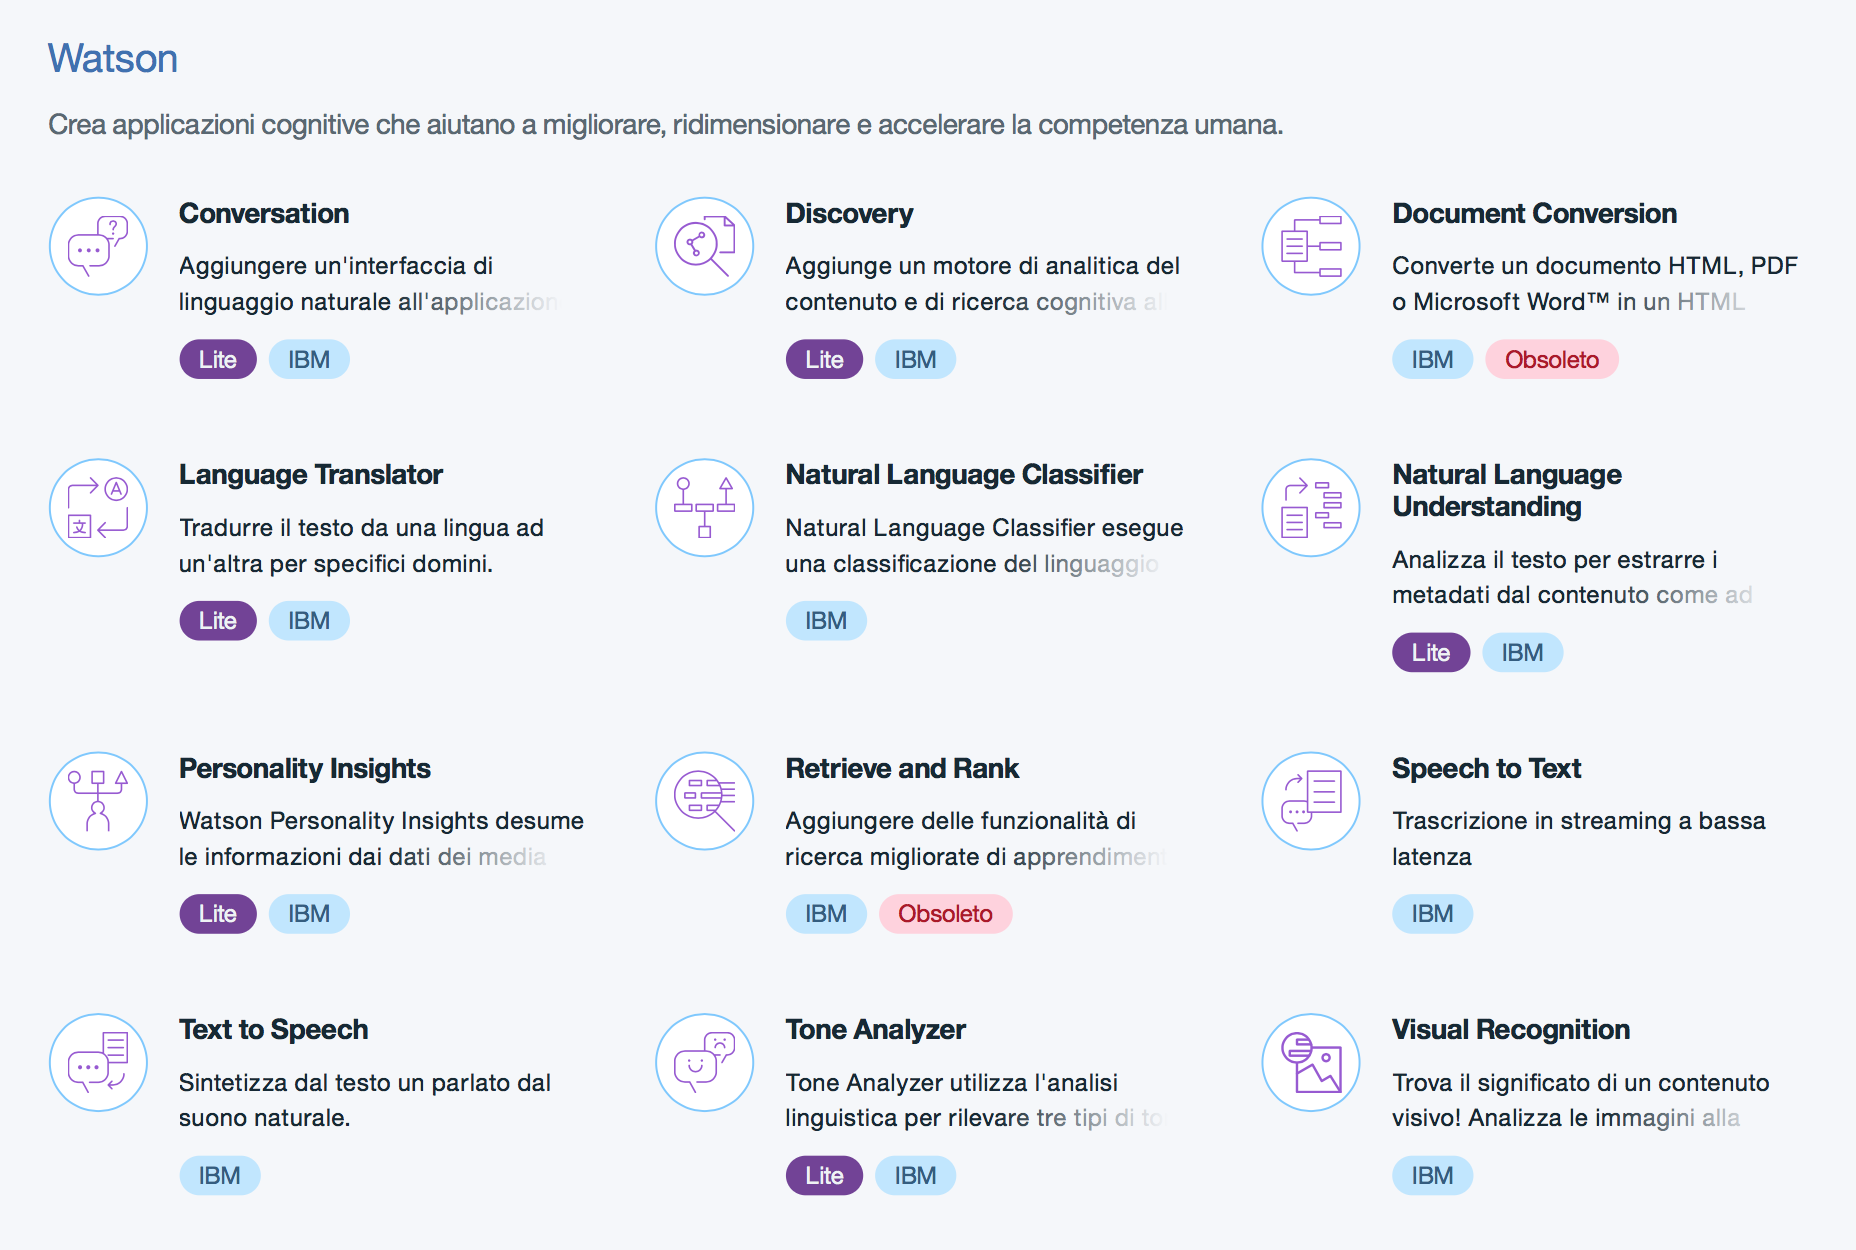
\includegraphics[width=\textwidth,keepaspectratio=true]{capitoli/imgs/watson.png}
	\caption{Alcuni moduli Bluemix appartenenti a Watson}
\end{figure}

\subsection{SaaS, Software as a Service}

Il Software as a Service (SaaS) è un modello di distribuzione del software in cui l'applicativo e gli eventuali servizi collegati sono eseguiti in un ambiente centralizzato e gli utenti vi accedono via rete, quasi sempre via Internet e usando un browser come interfaccia. I SaaS sono ormai sempre più diffusi. Tra i maggiori si ricordano le Google Apps (ad esempio Gmail, Google Drive, Google Calendar) e la suite Microsoft Office 365. Con la metodologia SaaS il provider fornisce tutto il software direttamente all'utente, al quale non resta che usarlo senza preoccuparsi di installazioni e configurazioni. L'utente non paga per il possesso del software, ma per il suo utilizzo. A volte vengono infatti applicate tariffe in base all'utilizzo del prodotto stesso. 

\paragraph{}
Spesso un'architettura SaaS è multi-tenant, ossia una sola applicazione server viene utilizzata da più utenti mantenendone, al tempo stesso, separati gli ambienti e i dati. Il concetto di multi-tenancy verrà approfondito maggiormente nei prossimi capitoli.
\paragraph{}
Attualmente le principali software house attive nel mondo aziendale traggono dalle offerte SaaS circa il venti percento del loro fatturato, nel giro di tre-quattro anni la maggior parte di loro prevede che il mercato SaaS diventi sempre più fondamentale.

\subsubsection{Vantaggi}
\paragraph{}
Con la metodologia SaaS il provider fornisce il software all'utente già pronto all'uso, l'utente non si deve quindi preoccupare di nient'altro. I clienti non pagano più per il possesso del software, ma per l'utilizzo dello stesso. In questo modo spesso possono essere notevolmente abbattute le spese iniziali per l'installazione e la configurazione di un prodotto, sostituendole con un costo di funzionamento. Il SaaS comporta quindi una spesa inferiore, ma ricorrente. E' il vendor però a preoccuparsi della manutenzione.
\paragraph{}
La caratteristica preponderante del cloud SaaS è proprio quella di poter raggiungere i propri dati personali da qualunque luogo e con qualunque dispositivo. E' questa la vera rivoluzione del cloud nel senso più comune del termine. Quando si ha bisogno di lavorare con i propri dati personali, non si ha più la necessità di avere con se hardware specifico, il proprio laptop o la propria usb key, ma basta avere le proprie credenziali al accedere così allo spazio dedicato. 
\paragraph{}
L'accesso alle tecnologie più sofisticate diviene inoltre alla portata di tutti. Software come gli ERP (Enterprise Resource Planning) e i CRM(Customer Relationship Management), possono essere utilizzati anche da quelle organizzazioni che prima non potevano permettersi un investimento di questo tipo.
\paragraph{} 
Un elemento che contraddistingue il SaaS è il notevole grado di apertura verso altre componenti, il che le rende altamente riusabili e flessibili, ciò è ovviamente un grande punto di forza in quanto i requisiti dell'utente spesso cambiano in continuazione.
\paragraph{}
Gli scenari di aggiornamento cambiano radicalmente. La distribuzione degli aggiornamenti è pressoché immediata e tutti gli utenti hanno la certezza di operare con l'ultima versione del software. Le fasi di upgrading non comportano più l'assenza del servizio come nella versione on premise. L'utente non si accorge neanche del processo di aggiornamento e si ritrova ad utilizzare il software aggiornato.
\subsubsection{Svantaggi}
\paragraph{}
Il modello ha ovviamente anche i suoi svantaggi, o perlomeno alcune criticità che vanno tenute presenti. La principale sta nella gestione dei dati aziendali, che sono localizzati nei data center del cloud provider e questo può essere giudicato un rischio per la privacy delle informazioni o addirittura costituire una violazione delle norme che devono osservare le aziende operanti in settori particolari come, ad esempio, la sanità e la difesa.
\paragraph{}
Tra gli altri aspetti di cui tenere conto ci sono sicuramente le prestazioni e l'affidabilità delle connessioni, che risultano essere i veri bottleneck non solo delle soluzioni SaaS, ma di tutte le soluzioni cloud. 
\paragraph{}
Infine altre criticità riguardano il provider dei servizi. Bisogna tenere conto quanto sia affidabile e se presenta, ad esempio, il rischio che esca dal mercato o ritiri il prodotto software SaaS. 

\begin{figure} [h!]
	\centering
	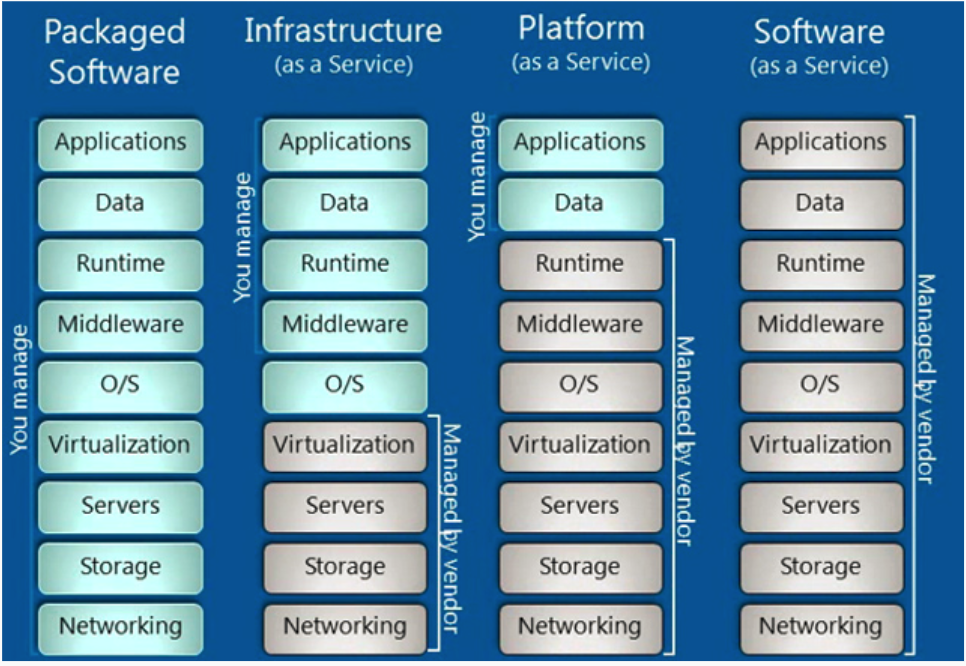
\includegraphics[width=0.7\linewidth]{capitoli/imgs/cloudstacks.png}
	\caption{Confronto di riepilogo tra i paradigmi cloud e il prodotto on premise}
\end{figure}


\section{SOA, Service Oriented Architecture}
Il concetto di Service Oriented Architecture è affine a quello di SaaS. Un SaaS può rappresentare la percezione da parte dell'utente della modalità di utilizzo di una Architettura Service Oriented. Un servizio ha l'obiettivo di incapsulare una ben precisa funzionalità, per renderla disponibile e accessibile come servizio software sul web. L'Architettura Orientata ai Servizi è quindi uno stile architetturale per la costruzione di una molteplicità di sistemi o applicazioni sulla base della composizione di un insieme di servizi. Spesso, quindi, queste applicazioni non fanno altro che comporre un SaaS, il quale trova in un'architettura di questo tipo una appropriata implementazione.
\section{Il software On Premise}
Abbiamo appena analizzato le peculiarità delle singole tipologie di servizi cloud. Anche il classico modello on premise però ha i suoi punti di forza.
\paragraph{Vantaggi del Software On Premise}
\begin{itemize}
	\item Controllo esclusivo su sistemi e dati
	\item Alta personalizzazione
	\item Gestione interna dei dati sensibili
	\item Alto investimento iniziale ammortizzato nel lungo periodo
\end{itemize}

\paragraph{}
Nel caso in cui si abbiano già a disposizione tutte le infrastrutture necessarie, non risulta più vero che la soluzione cloud sia la più economica per far fronte alla necessità di un determinato applicativo. E' anche necessario però che il software sia abbastanza centralizzato per adottare una soluzione on premise e questo può rappresentare un rischio per la fault tolerance.

\paragraph{}
Occorre quindi fare un'analisi di quanto sia necessario personalizzare il software di cui si ha bisogno e averne il pieno controllo come nella modalità onpremise, tenendo conto che un software on premise richiede molta più cura, manutenzione e lavoro di una soluzione basata su cloud. Il paradigma di fornitura on premise risulta ancora essere la soluzione più adatta nel caso in cui la gestione diretta dei dati sia fondamentale per policy aziendali oppure sia necessaria una maggiore flessibilità di configurazione per l'integrazione con altre architetture software. Un'altro requisito che ne può richiedere l'adozione è la necessità che l'architettura fisica del software sia geograficamente centralizzata.

  \chapter{SaaS, le tecnologie che ne consentono la realizzazione}

\section{SaaS e i suoi requisiti}

\subsection{Availability}
Il concetto di Availability, nel senso generale del termine, è ben definito dallo standard ITU-T E.800: "L'abilità di un sistema di essere in uno stato che soddisfa un determinato requisito, in determinati istanti di tempo, assumendo che le risorse a lui necessarie siano disponibili." Come possiamo vedere, è un concetto ben definito, ad ha quindi le sue metriche ben definite che quantificano l'Availability. 

\paragraph{MTTF, Mean Time TO Failure}
Misura l'intervallo di tempo tra due eventi di "faiulure", in cui il sistema non è riuscito a portare a termine il proprio compito.

\paragraph{}
Possiamo dire quindi che l'Availability rappresenta la porzione di tempo in cui il sistema si comporta secondo le proprie specifiche. Va tenuto in considerazione anche che, al verificarsi di un fallimento, al tempo di non-Availability si aggiunge il tempo per porre rimedio al fallimento e far ripartire il sistema. 

\paragraph{}
Possiamo immaginare, a questo punto, quanto sia fondamentale un'altissima availability per i servizi Cloud 


  \chapter{SaaS, le tecnologie che ne consentono la realizzazione}
Nel corso degli ultimi anni, con il proliferare delle piattaforme e dei servizi di cloud computing, sono nate e si sono sviluppate molte tecnologie per soddisfare le nuove esigenze e i nuovi requisiti appena visti che questa rivoluzione della fruizione del software ha comportato.

\section{Microservizi}
Un concetto fondamentale, di cui il Cloud Computing fa largamente uso, sono i mircoservizi. Cominciamo col darne una definizione abbastanza formale: "Lo stile architetturale a microservizi è un approccio allo sviluppo di una singola applicazione come insieme di piccoli servizi, ciascuno dei quali viene eseguito da un proprio processo e comunica con un meccanismo snello, spesso una HTTP API.(Martin Fowler)".

\paragraph{}
L'approccio è quello di dividere le funzionalità del sistema in più microservizi. Ad ogni microservizio corrisponde una necessità dell'utente. La filosofia di dividere il software in base alle responsabilità è già presente da tempo nell'ingegneria del software. Una suddivisione modulare del sistema in base ai casi d'uso dell'utente è un dogma dell'Object Oriented Design, ma la novità apportata dai microservizi è che il sistema risulta scomposto in piccoli servizi che sono completamente indipendenti tra loro. Ogni microservizio si preoccupa infatti di risolvere un particolare problema del cliente, un unico scenario. La comunicazione tra i servizi avviene attraverso la rete al fine di garantire l'indipendenza tra i servizi ed evitare ogni forma di accoppiamento. Ogni microservizio, infatti, rappresenta un'entità separata che generalmente può essere pubblicata come un modulo di una Platform as a Service.

\subsection{Il modello monolitico a layer }
Secondo il classico modello a layer le funzionalità vengono suddivise tra i diversi livelli in base al grado di astrazione, usando delle tecnologie proprie di ogni livello. Con questa architettura però, nonostante ci sia una suddivisione a strati, il software risulta essere un unico sistema monolitico, sebbene molti componenti possano essere comunque riusabili.

\begin{figure}[h!]
	\centering
	
\includegraphics[width=\textwidth,keepaspectratio=true]{capitoli/imgs/disegnoMicrosMonol.png}
	\caption{Il modello monolitico e i microservizi}
\end{figure}

\subsection{Confronto tra l'architettura a microservizi e il modello monolitico}
La scelta di adottare uno o l'altro approccio viene dopo un'attenta analisi dei requisiti che il sistema deve soddisfare. In questo studio però va anche tenuto conto quanto le esigenze possano cambiare nei futuri utilizzi del software.
\begin{itemize}
	\item La struttura interna di tutto un sistema monolitico è composta dai layer di interfacciamento con l'utente, logica di business e persistenza dei dati. In un'architettura a microservizi non troviamo questa divisione a livello di sistema, ma la ritroviamo semmai all'interno di ogni singolo microservizio atomico. Il microservizio si occuperà, ad esempio, di preservare il suo stato tramite l'utilizzo di un proprio database non condiviso con gli altri microservizi. 
	
	\item Uno dei fattori chiave da considerare è la scalabilità. Per scalare un'applicazione monolitica occorre necessariamente clonarla in più server, macchine virtuali o contenitori.
	
	\item Quando occorre scalare orizzontalmente un'architettura a microservizi, si creano e si distribuiscono indipendentemente tra loro repliche dei microservizi in più server o container. 
\end{itemize}


\begin{figure}[h!]
	\centering
	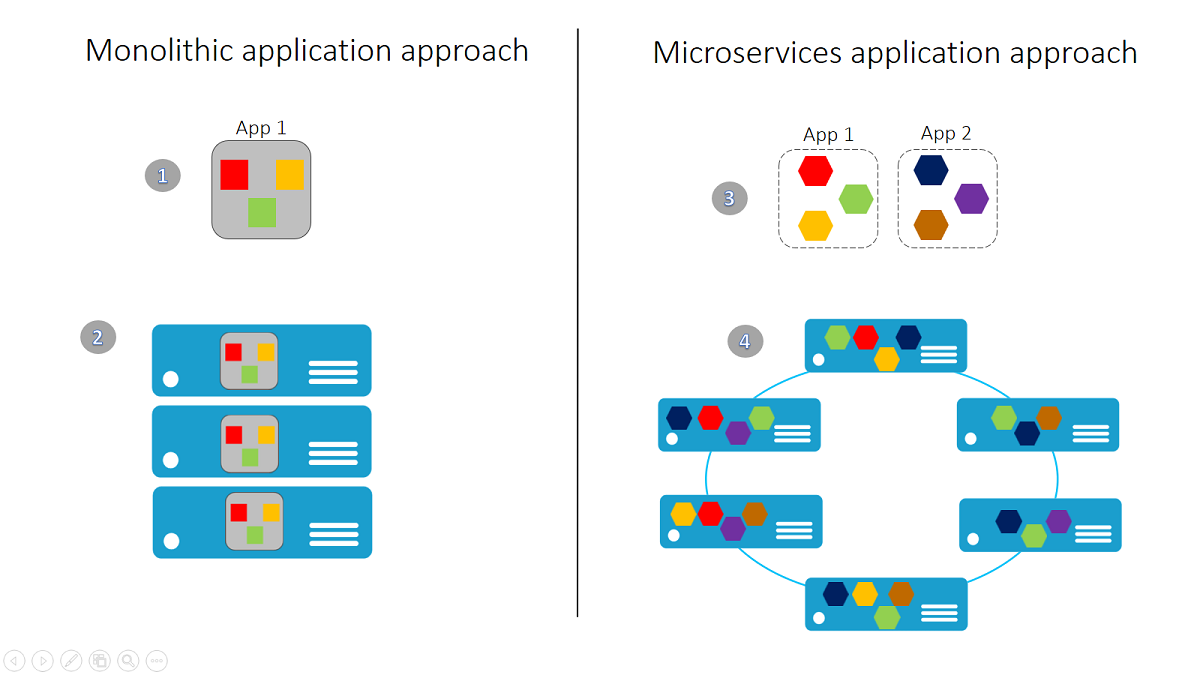
\includegraphics[width=\textwidth,keepaspectratio=true]{capitoli/imgs/monosvmicro.png}
	\caption{Il modello monolitico e i microservizi}
\end{figure}

\subsection{Vantaggi e svantaggi di un'architettura a microservizi}
Un'architettura di questo tipo porta con se ovviamente anche i suoi svantaggi e i suoi vantaggi. Andiamo a vedere come questi ultimi corrispondano proprio alle esigenze del cloud computing.

\subsubsection{Vantaggi}
\begin{itemize}
	\item  Velocità \\
	L'architettura a microservizi è quella che si sposa meglio con la metodologia agile. un microservizio deve avere sempre delle dimensioni ridotte e il suo sviluppo ha una durata di circa due settimane. Ciò porta ad avere fin da subito piccole porzioni del sistema (i servizi appunto), pronte, testabili ed utilizzabili. Ogni microservizio inoltre è autonomo e può quindi giungere in ambiente di produzione indipendentemente dagli altri. In questo modo si riesce a reagire molto velocemente alle esigenze di mercato.
	
	\item Sperimentazione \\
	Con i microservizi la modularità del sistema è un notevole punto di forza. Sperimentare nuove tecnologie all'interno di un singolo microservizio ha un impatto nullo su tutti gli altri. Si è in questo modo molto più invogliati a ricercare sempre più nuove tecnologie da inserire nel proprio prodotto. Il rischio è minimo in quanto, anche nel caso l'esperienza risulti fallimentare, la mole di lavoro che comporta la modifica di un microservizio è veramente molto ridotta.
	
	\item Tecnologie ad hoc \\
	Altro fattore da considerare è la possibilità di differenziare le tecnologie a seconda del microservizio. Si prenda come esempio la vastità di tipologie di database che sono disponibili all'uso. Un database che è appropriato per un microservizio potrebbe non essere la scelta migliore per un altro. 
	
	\item Scalabilità \\
	I software con un'architettura a microservizi sono pensati per scalare orizzontalmente in maniera estremamente agevole. Si possono replicare a piacimento tramite l'utilizzo di containers e hanno un comportamento distribuito anche nel caso si trovino sulla stessa macchina, in quanto i container li isolano da tutti gli altri.
	
	\item Facilità di Deployment \\
	Le modifiche hanno un impatto molto ridotto nell'intero sistema. Grazie a ciò è possibile rilasciare sul mercato il software aggiornato con frequenze molto maggiori. Potenzialmente ogni modifica può subito essere pubblicata e non occorre attenersi a lunghi processi di release in cui si cerca il più possibile di accumulare modifiche da effettuare per poi applicarle tutte insieme.
	
	\item Portabilità \\
	Il software a microservizi è facilmente componibile e portabile su più contesti e dispositivi, come quello web, mobile ma anche sistemi embedded, dispositivi indossabili e molto altro.	
\end{itemize}

\subsubsection{Svantaggi}
\begin{itemize}
	\item Dipendenza dalla rete \\
	E' questo il principale punto di critico di un'architettura a microservices. Abbiamo visto quanto l'interazione tra i singoli microservizi faccia affidamento su una comunicazione attraverso la rete. Ovviamente questo deve essere un requisito fondamentale. In mancanza di una connessione adeguata tutto il sistema smette di funzionare correttamente.
	
	\item Identità e autenticazione \\
	Una volta che un utente effettua il login al sistema occorre garantire che la sua autenticazione, e soprattutto la sua identità, venga mantenuta in tutti i microservizi che andranno a comporre la sua esperienza utente.
\end{itemize}

\section{Containers}
I container sono l'habitat naturale dei microservizi. Essi forniscono al software tutto ciò che gli è necessario, garantendogli un ambiente estremamente leggero e flessibile.

\begin{figure}[h!]
	\centering
	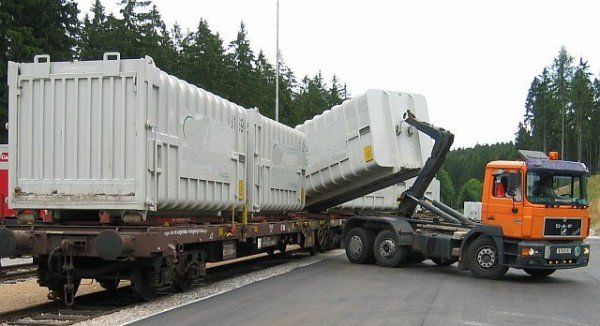
\includegraphics[width=\textwidth,keepaspectratio=true]{capitoli/imgs/spostamentocontainer.png}
	\caption{Containers nell'accezione dell'industria dei trasporti}
\end{figure}

\paragraph{}
La parola container vuole alludere ad una analogia con l'attrezzatura specifica dei trasporti. Da dove è nata la necessità dell'utilizzo dei container? Immaginiamo lo scenario in cui alcune merci andassero trasportate prima via terra, magari con un camion, e poi via mare per raggiungere un altro stato. Prima dell'avvento dei container il camion arrivava al porto, andava aperto e il contenuto passato in un mercantile pronto sul molo. L'operazione era effettuata manualmente e i singoli imballaggi erano trasbordati uno alla volta con grande dispendio di tempo e mezzi. Si è iniziato allora a considerare più pratica l'idea di trasbordare sulla nave l'intero corpo del camion. Nacquero così i container: contenitori multiuso, realizzati in formati standard che possono essere passati con facilità da un camion a una nave e poi magari su un treno merci e così via.

\paragraph{}
E così anche nel nostro caso abbiamo bisogno di uno strumento che possa contenere i microservizi e le applicazioni, che ci consenta di manovrarle con facilità senza sapere cosa facciano esattamente.
I containers sono infatti un metodo di virtualizzazione del sistema operativo che ha come obiettivo quello di isolare il software che ospita, permettendo di eseguire le applicazioni e le loro dipendenze in processi completamente isolati. L'infrastruttura del container interagisce direttamente con il kernel della macchina che lo ospita, scavalcando gli altri layer. In qualsiasi sistema operativo collochiamo il container, le sue configurazioni interne rimarranno sempre separate, e l'applicazione contenuta si troverà garantito il suo ecosistema necessario all'esecuzione. Non ci si deve preoccupare, ad esempio, di produrre una versione software per Windows e una per sistemi UNIX, ma la soluzione a container è unica e portabile. 

\begin{figure}[h!]
	\centering
	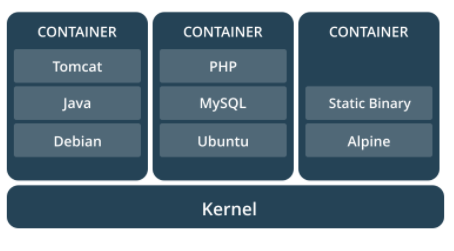
\includegraphics[width=\textwidth,keepaspectratio=true]{capitoli/imgs/container.PNG}
	\caption{Schematizzazione di tre container sulla stessa macchina ospitante}
\end{figure}

\subsection{I containers e le Macchine Virtuali}
Stando alla descrizione dei container che abbiamo dato fino a questo punto potrebbe sorgere una domanda: perché utilizzare i container se potrebbero essere comodamente usate delle macchine virtuali? Una Virtual Machine è per sua natura già isolata dalla macchina che la ospita. La risposta sta nella leggerezza d'uso dei container. I container infatti non virtualizzano l'hardware della macchina, ma solamente il layer applicativo, rendendoli più portabili ed efficienti.

\paragraph{}
Non avendo un proprio sistema operativo, il peso di un container e dell'ordine di qualche Megabyte, contro i Gigabyte di una macchina virtuale che sovrappone il proprio sistema operativo a quello della macchina ospitante. A differenza delle macchine virtuali inoltre, i container non necessitano dell'Hypervisor, un componente che svolge delle attività di controllo e coordinamento sulle macchine virtuali. 

\begin{figure}[h!]
	\centering
	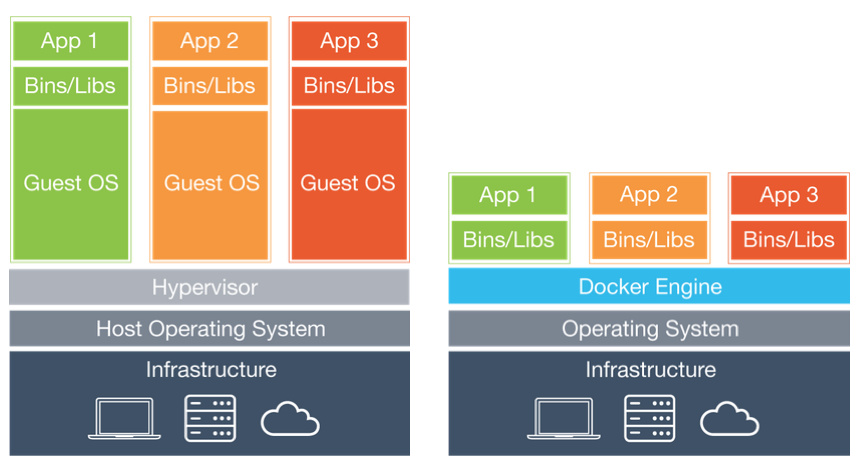
\includegraphics[width=\textwidth,keepaspectratio=true]{capitoli/imgs/ContainersvsVms.PNG}
	\caption{Confronto tra macchine virtuali e container, nell'esempio con l'utilizzo di un Docker Engine}
\end{figure}

\subsection{Vantaggi dei container}
Andiamo a ricapitolare quali sono le principali motivazioni che possono spingerci verso l'adozione dei container.
\begin{itemize}
	\item Coesione dell'ambiente \\
	L'ambiente di un container è fortemente disaccoppiato dalla macchina in cui si trova. Questo fa si che il proprio contenuto sia facilmente replicabile e portabile ovunque.
	
	\item Gestione delle risorse \\
	Con i container si ha una gestione delle risorse di calcolo molto più efficiente. Richiedendo poche risorse alla macchine ospitante, si ha la possibilità di eseguire molti più container contemporaneamente. 
	
	\item Produttività \\
	Diminuendo le dipendenze, ci si alleggerisce di tutta la mole di lavoro necessaria per configurare correttamente un prodotto. 
	
	\item Gestione degli aggiornamenti. \\
	Molto spesso la gestione degli aggiornamenti è un meccanismo già compreso nei container engine, come Docker.
\end{itemize}

\subsection{I container e i microservizi}
Possiamo quindi comprendere come i container siano estremamente appropriati ad ospitare dei microservizi. Ponendo un microservizio dentro un container, abbiamo la garanzia che ogni microservizio operi come un sistema separato, anche nell'eventualità che due servizi risiedano nella stessa macchina fisica. Ogni microservizio inserito in un container gode automaticamente di tutti i vantaggi di portabilità e flessibilità dei container che sono tra i requisiti fondamentali che ci spingono verso l'architettura a microservizi.

\subsection{Docker}

\begin{figure}[h!]
	\centering
	
\includegraphics[width=\textwidth,keepaspectratio=true]{capitoli/imgs/docker.png}
	\caption{Logo di Docker}
\end{figure}

\paragraph{}
Docker è una piattaforma open source nata nel 2013 e scritta in linguaggio Go. Il suo scopo è quello di facilitare ed automatizzare il deployment delle applicazioni all'interno dei container. Il tool offre allo sviluppatore delle comode API di gestione che consentono agli sviluppatori di testare le applicazioni, effettuare build e distribuire il proprio prodotto. Docker fa utilizzo di numerose librerie come, ad esempio, libcontainer che ha lo scopo di interagire con il kernel di Linux.  In questo modo, isolando risorse, servizi e processi, dalla prospettiva dell'utilizzatore del container si ha l'impressione di un utilizzo esclusivo del sistema operativo.

\paragraph{}
Il container diviene con Docker l'unità di distribuzione del prodotto. Quando il servizio è stato correttamente implementato, è pronto per essere distribuito e, attraverso il container, può essere inserito in un orchestratore per garantirne il ciclo di vita.

\paragraph{Docker Engine}
L'Engine di Docker è una struttura a strati, troviamo:
\begin{itemize}
	\item Il server, un demone chiamato dockerd che è sempre in running. E' il componente che crea e gestisce gli oggetti Docker.
	\item Le REST API, che rappresentano l'interfaccia per interrogare il server.
	\item La Command Line Interface, che è quella con la quale si interfaccia l'utente e si aggancia alla REST API.
\end{itemize}

\begin{figure}[h!]
	\centering
	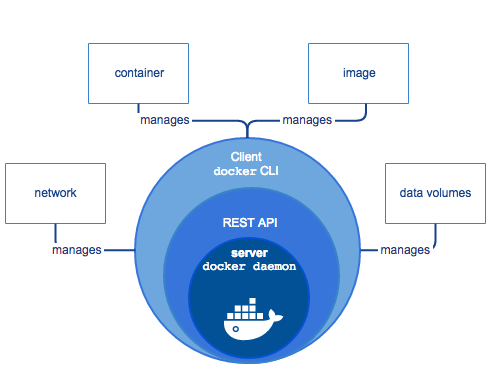
\includegraphics[width=\textwidth,keepaspectratio=true]{capitoli/imgs/dockerThinking.png}
	\caption{Docker engine}
\end{figure}

\paragraph{Architettura di Docker}
L'architettura di Docker è una classica architettura client-server. Il client parla direttamente con il Docker daemon che si trova sul server. E' proprio il dockerd che si prende l'onere di fare gran parte del lavoro, quello di far partire e distribuire i container.
\begin{figure}[h!]
	\centering
	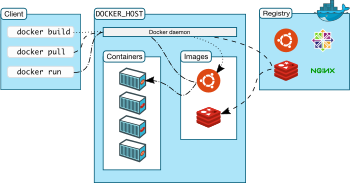
\includegraphics[width=\textwidth,keepaspectratio=true]{capitoli/imgs/architecturedocker.png}
	\caption{Architettura di Docker}
\end{figure}
\paragraph{}
I componenti che vanno a costituire l'architettura di Docker sono i seguenti:
\begin{itemize}
	\item Docker deamon \\
	Abbiamo già parlato di lui. Dockerd è in ascolto di chiamate da parte della REST API. E' sua responsabilità far funzionare tutto l'engine della gestione dei container.
	\item Docker client \\
	Lo scopo principale del client è interagire con chi sviluppa il contenuto dei container. Questo componente recepisce i comandi da parte dello sviluppatore e li traduce in chiamate per il deamon.
	\item Docker registries \\
	Sono i registri che consentono di conservare le immagini di Docker. Immaginiamo che sia interesse di chi li sviluppa poter conservare e mettere in vendita servizi implementati all'interno dei container. Vengono offerte anche delle comode API e uno store nel quale mettere a disposizione le proprie immagini.
	\item  Docker objects \\
	In questa categoria rientrano più tipologie di oggetti Docker, come quelli che andiamo ad analizzare qui di seguito. \begin{itemize}
		\item  Images \\
		Un'immagine è un template standard che si utilizza per parametrizzare un nuovo container che si sta per mettere in piedi. Per creare la propria immagine, con i parametri personalizzati, si dichiarano nel Dockerfile gli step necessari. Successivamente ad ogni step corrisponderà a un layer del container.
		\item  Container \\
		Un container è l'istanziazione di una immagine, esso infatti è definito univocamente dalla propria immagine. E' un elemento che può essere gestito a piacimento e può essere collegato ad una o più reti, fattore importantissimo per far interagire il proprio contenuto con quello di altri container.
		\item Services \\
		I servizi permettono di scalare i container attraverso più Docker deamon. In questo modo si riesce a dare ugualmente l'impressione all'utente di utilizzare un servizio esclusivo e centralizzato.
	\end{itemize}
\end{itemize}

\subsection{Kubernetes}
\begin{figure}[h!]
	\centering
	
\includegraphics[width=\textwidth,keepaspectratio=true]{capitoli/imgs/kubernetes_full.png}
	\caption{Logo di Kubernetes}
\end{figure}

\paragraph{}
Abbiamo appena tessuto le lodi di Docker. Ora però poniamoci alcune domande: come possono essere coordinati, distribuiti e gestiti i container e il loro workload, man a mano che vengono consumate le risorse disponibili nell'infrastruttura sottostante? Come operano i container in un ambiente network multi-tenant? Quale livello di sicurezza propone Docker? E chi decide quale sia il giusto livello di astrazione?

\paragraph{}
Per far fronte a queste necessità è nato da Google nel 2014 Kubernetes. Esso offre un layer di astrazione per migliorare le performance dei container stessi eliminando molti dei processi manuali coinvolti nel deployment e nella scalabilità di applicazioni containerizzate. Consente di far cooperare opportunamente insiemi di container componendo delle unità logiche utili nelle nostre applicazioni.

\paragraph{Perché utilizzare Kubernetes?}
Le applicazioni di produzione si espandono spesso su più container, questi devono essere distribuiti a loro volta su diversi server host. Kubernetes offre le capacità di orchestrazione e gestione necessarie per distribuire i container, in modo scalabile, al fine di gestire i carichi di lavoro. L'orchestrazione di Kubernetes consente di creare servizi che si estendono su più container, gestirne la scalabilità e l'integrità nel tempo.

\begin{figure}[h!]
	\centering
	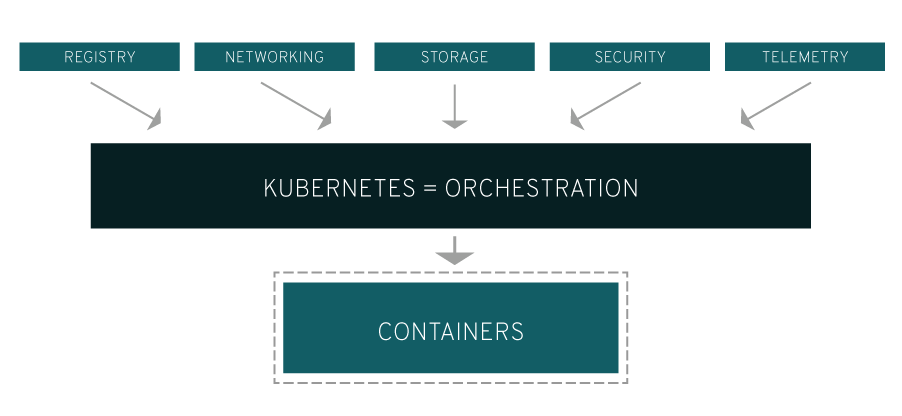
\includegraphics[width=\textwidth,keepaspectratio=true]{capitoli/imgs/kubernetes-diagram.png}
	\caption{Ruolo di orchestratore di Kubernetes}
\end{figure}

\paragraph{I Pod di Kubernetes, cosa sono?}
Kubernetes risolve molti dei noti problemi relativi alla proliferazione dei container, raggruppandoli in un pod. I pod aggiungono quindi un livello di astrazione ai cluster di container. La loro funzione è quella di alleggerire i carichi di lavoro e fornire i servizi necessari, tra cui rete e storage, ai container stessi. Kubernetes agevola, inoltre, il bilanciamento del carico all'interno dei pod e garantisce l'utilizzo di un numero di container adeguato per supportare i carichi di lavoro.

\paragraph{Architettura di Kubernetes}
\begin{figure}[h!]
	\centering
	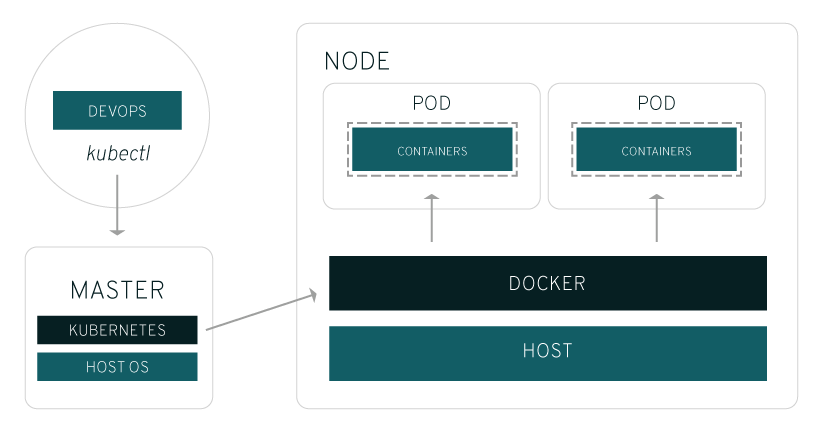
\includegraphics[width=\textwidth,keepaspectratio=true]{capitoli/imgs/kubernetesarchitetcture.png}
	\caption{Architettura di Kubernetes}
\end{figure}

Andiamo a definire quelli che sono i termini di riferimento in Kubernetes:
\begin{itemize}
	\item Master \\
	E' la macchina che controlla i nodi Kubernetes. È il punto di origine di tutte le attività assegnate.
	\item Nodi \\
	Queste macchine eseguono le attività assegnate richieste. Sono controllate dal nodo master di Kubernetes. Possono essere assimilate con gli host dei container.
	\item Pod \\
	Rappresenta un gruppo di uno o più container distribuiti su un singolo nodo. Tutti i container presenti in un pod condividono indirizzo IP, IPC, nome host ed altre risorse. I pod astraggono la rete e lo storage dal container sottostante, consentendo di spostare i container nei cluster con maggiore facilità.
	\item Service \\
	Questa componente ha la funzionalità di disaccoppiare le definizioni del lavoro dai pod.
	\item Kubelet \\
	Questo servizio viene eseguito sui nodi, legge i manifest del container e garantisce che i container definiti vengano avviati ed eseguiti.
	\item Kubctl \\
	Questo componente si interfaccia direttamente con il programmatore. Presenta una riga di comando per la creazione e gestione dei pod.
\end{itemize}

\paragraph{E Docker?}
La piattaforma docker mantiene le proprie funzioni. Quando Kubernetes assegna un pod ad un nodo, il kubelet su quel nodo chiede a docker di lanciare i container specificati. Quindi, il kubelet legge continuamente lo stato di quei container da docker e aggrega le informazioni nel nodo master. Docker invia i container sul nodo e avvia e arresta opportunamente i container. La differenza con lo scenario senza Kubernetes è che un sistema automatizzato con Kubernetes chiede a docker di eseguire queste operazioni, anziché assegnarle ad un amministratore, il quale deve eseguirle manualmente su tutti i nodi, in tutti i container.

\section{Multitenancy}
La multitenancy è un paradigma che, andando a braccetto con il cloud computing, si sta diffondendo sempre di più nel panorama delle architetture software. Esso prevede che una singola istanza del software in questione, situato su un server, sia utilizzato da molti utenti, chiamati tenant. I tenant condividono l'accesso comune al servizio con privilegi differenziati sulle istanze software. L'obiettivo principale è quello di garantire scalabilità al servizio e dare al tenant la percezione di un possesso esclusivo del software.
\begin{figure}[h!]
	\centering
	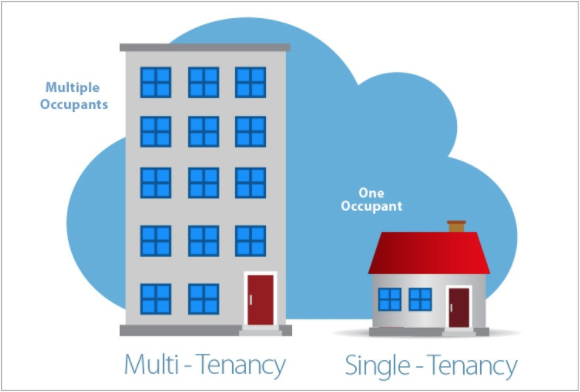
\includegraphics[width=0.7\textwidth,keepaspectratio=true]{capitoli/imgs/multitenancy.png}
	\caption{Esempi di Multitenancy e Single-Tenancy per il contesto abitativo}
\end{figure}

\paragraph{Vantaggi della Multitenancy}
\begin{itemize}
	\item Costi \\
	Scalare un'architettura multitenant è più economico, in quanto si interviene solamente in un'unica macchina fisica e acquistare hardware più performante risulta meno dispendioso. Inoltre in questo modo si riduce anche il numero di licenze da acquistare, nel caso siano necessarie.
	\item Data Mining \\
	Nel caso sia necessario estrapolare dei dati da tutti i clienti, avere dei tenant tutti sulla stessa macchina rende l'operazione molto più immediata.
	\item  Release Management \\
	Al rilascio di una nuova versione il processo risulta essere molto semplificato. Ciò viene ovviamente dal fatto che dovendo aggiornare una sola istanza del software su una sola macchina fisica la mole di lavoro è sicuramente minore.
\end{itemize}

\paragraph{Requisiti}
Ovviamente un'architettura multitenant ha anche dei requisiti. Nonostante l'unicità del software, si deve garantire un alto grado di "personalizzazione" ai diversi tenant, proprio come se avessero un utilizzo esclusivo del servizio. Da un altro lato ci si aspettano elevati parametri di security, robustezza e prestazioni.

\section{DevOps, Continuous Delivery e Continuous Integration}

\section{Monitoring Tools}
La centralizzazione portata dal SaaS comporta anche un radicale cambiamento delle modalità di monitoring del sistema. Non è pensabile che una persona possa andare a controllare tutti i log dei servizi e misurare le prestazioni degli stessi manualmente. E' necessario l'utilizzo di appositi tool che hanno come finalità quella di raccogliere questa mole di informazioni, elaborarle e presentarle al personale addetto del provider nel modo più intellegibile possibile. In questa ottica andiamo a presentare due tool utilizzati nel progetto BigFix SaaS: Prometheus e Grafana.
\subsection{Prometheus}
\begin{figure}[h!]
	\centering
	
\includegraphics[width=0.5\textwidth,keepaspectratio=true]{capitoli/imgs/prometheuslogo.png}
	\caption{Logo di Prometheus}
\end{figure}
\paragraph{}
Prometheus è un tool di monitoring open-source nato nel 2012 e scritto in Go. Si adatta sia alle architetture centralizzate che a quelle distribuite. La struttura del tool è pensata per garantire un validissimo supporto nel caso il servizio monitorato abbia dei malfunzionamenti. Vediamo un elenco delle caratteristiche principali.
\begin{itemize}
	\item Un data model multidimensionale che ha lo scopo di raccogliere tutti i dati.
	\item Un query language flessibile per far fronte a questi dati.
	\item Engine per la rielaborazione dei dati.
	\item Meccanismi sofisticati per collezionare serie storiche.
	\item Supporto per le dashboard.
\end{itemize}
\subsection{Grafana}
\begin{figure}[h!]
	\centering
	
\includegraphics[width=0.3\textwidth,keepaspectratio=true]{capitoli/imgs/grafanalogo.png}
	\caption{Logo di Grafana}
\end{figure}
Grafana consente di avere una finestra da cui monitorare tutti i servizi in maniera centralizzata. Consente di visualizzare dati, creare degli alert e visualizzare tutte le informazioni in comode interfacce per gli utenti.
\begin{figure}[h!]
	\centering
	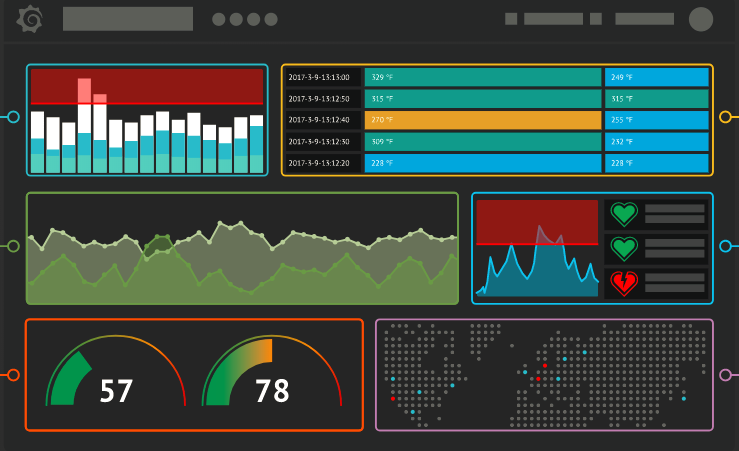
\includegraphics[width=0.7\textwidth,keepaspectratio=true]{capitoli/imgs/grafanainterface.PNG}
	\caption{Una delle interfacce di Grafana}
\end{figure}
\section{BlueMix Services}
\begin{figure}[h!]
	\centering
	
\includegraphics[width=0.7\textwidth,keepaspectratio=true]{capitoli/imgs/bluemixlogo.png}
	\caption{Logo di IBM BlueMix}
\end{figure}
Come abbiamo accennato precedentemente, IBM BlueMix è una PaaS che offre molti microservizi utili per il cloud computing. Il vantaggio dei microservizi è che possono essere utilizzati a piacimento in qualsivoglia progetto, come nel nostro caso. Alcuni dei servizi BlueMix sono stati anche utilizzati nel nostro progetto e altri lo saranno in seguito, con degli sviluppi futuri.
\paragraph{}
Ne sono un esempio il database DB2 e Kubernetes, che nel nostro caso sono stati integrati utilizzando le loro versioni presenti su BlueMix. E' possibile inoltre che in futuro si adotti un'altro database IBM sempre presente su BlueMix, Cloudant, un database NoSQL nativo cloud.

  \chapter{IBM BigFix Detect on SaaS, realizzazione del prototipo}

\section{Interaction Design}

  \chapter{IBM BigFix on SaaS, l'implementazione del prototipo}
L'attenta progettazione giudata dall'architect che abbiamo visto nel capitolo precedente è servita da base per la vera ralizzazione del prototipo che rappresenta l'aspetto implementativo del progetto BigFix SaaS. Ma queste due fasi del lavoro che stiamo presetando non sono l'una successiva l'altra. Infatti è bene rimarcare che, sguendo un approccio agile, iterativo e incrementale, l'intero disegno del progetto si è ottenuto solamente a fronte di una continua esplorazione dei requisiti che si è protratta durante tutta la fase implementativa. Il metronomo dello sviluppo sono state infatti le sprint demo, le quali vedevano la partecipazione anche di altri stackeholders interni all'azienda, oltre che al team stesso. Da questi confronti sono risultati continui feedback che hanno contribuito a portare il lavoro nel suo stato attuale.

\section{Container e microservizi di BigFix}
Per la necessità di continui feedback già dalla prima fase del progetto si è scelto di adottare, per i primi sprint, una soluzione intermedia per quanto riguarda la scomposizione del prodotto nei container. Si deciso infatti di fare in modo che, all'inizio, ogni container ospitasse un realay o un server di uno dei clienti forniti dal SaaS, e non un microservizio vero e proprio del prodotto. Questa scelta è avvenuta dopo un analisi dei requisiti. Scomporre BigFix in microservizi è un'operazione che richiede molte ore uomo di lavoro e affrontarla all'inizio del progetto non avrebbe consentito ti testare nelle primissime fasi le tecnologie che si erano individuate per il deployment. Avendo presto a disposizione gli ambienti cliente con relay e server, si sono subito testati scenari tipici del prodotto on premises nelle nuove tecnologie SaaS adottate.

\section{Gli ambienti di sviluppo }
La realizzazione di un progetto aziendale richiede più ambienti nei quali, sequenzialmente, viene testato il prodotto prima di metterlo sul mercato. L'ambiente ufficiale, quello di produzione, deve garantire tutti i parametri qualitativi di cui abbiamo parlato precedentemente. Per questo motivo è lì che si concentrano i maggiori investimenti a livello hardware per garantire alte prestazioni al servizio. Al tempo stesso però occorre avere a disposizione un "laboratorio" in cui sviluppare e testare il software, in cui implementare le nuove features quando il prodotto sarà già sul mercato, un ambiente nel quale le modifiche che si compiono al codice non impattino in nessun modo il servizio offerto ai clienti. Per questo motivo il primo contesto in cui si è andato a lavorare è l'ambiente di sviluppo. Un ambiente chiuso all'esterno dell'azienda, ma che al tempo stesso simulasse nella maniera più fedele possibile l'ambiente di produzione. A questi due si aggiunge un'ambiente intermedio di pre production, nel quale vengono svolti tutti i test qualitativi per verificare che il prodotto sia conforme ai parametri non funzionali stabiliti. 
\begin{figure}[h!]
	\centering
	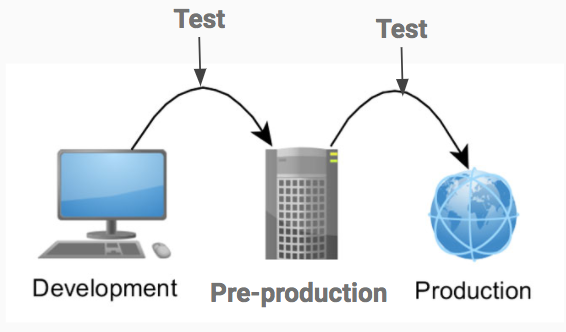
\includegraphics[width=0.7\textwidth,keepaspectratio=true]{capitoli/imgs/ambientisviluppo.png}
	\caption{Ambienti di BigFix SaaS}
\end{figure}

\section{Costruzione dell'ambiente e installazione di Docker e Kubernetes}
Vediamo una schematizzazione dell'ambiente di sviluppo nella figura \ref{ambs}. Kubernetes è il tool che muove le danze avendo proprio la funzione di orchestratore dei container. L'architettura di Kubernetes richiede che ci sia un nodo master che coordina i nodi denominati kube-node, che possono rappresentare macchine diverse. Su tutti i kube-node è installato anche docker, in quanto ci permetterà di ospitare su di essi i container. Questi vengono deployati su tutti i nodi a disposizione seguendo l'algoritmo di scheduling round-robin in modo da gestire al meglio le risorse di calcolo. 
\paragraph{}
Il Kubernetes master si interfaccia, come posiamo vedere, anche con altre due macchine presenti nella rete: La macchina DB2 e la macchina NFS. Andiamo a vedere di cosa si tratta.
\paragraph{DB2}
E' la macchina che ospita una replica del database. Spiegheremo in seguito come, nel processo di onboarding di un nuovo cliente, vengono dinamicamente allocate le risorse del database al nuovo utente. Le modalità di interazione tra i componenti BigFix nei container e il database ricalcano quelle del prodotto on premise.
\paragraph{Network File System (NFS)}
Questo componente è pensato per fornire storage per i container tramite protocollo NFS. L'NFS è un protocollo di rete sviluppato dalla Sun negli anni 80. Esso rappresenta un file system distribuito che consente ai computer di utilizzare la rete per accedere ai dischi rigidi remoti come fossero dischi locali. La componente NFS è stata utilizzata solamente in una prima fase del progetto in quanto, con il passaggio all'ambiente ufficiale, si è fatto affidamento allo storage fornito da un particolare componente di Kubernetes, il service. 

\begin{figure}[h!]
	\centering
	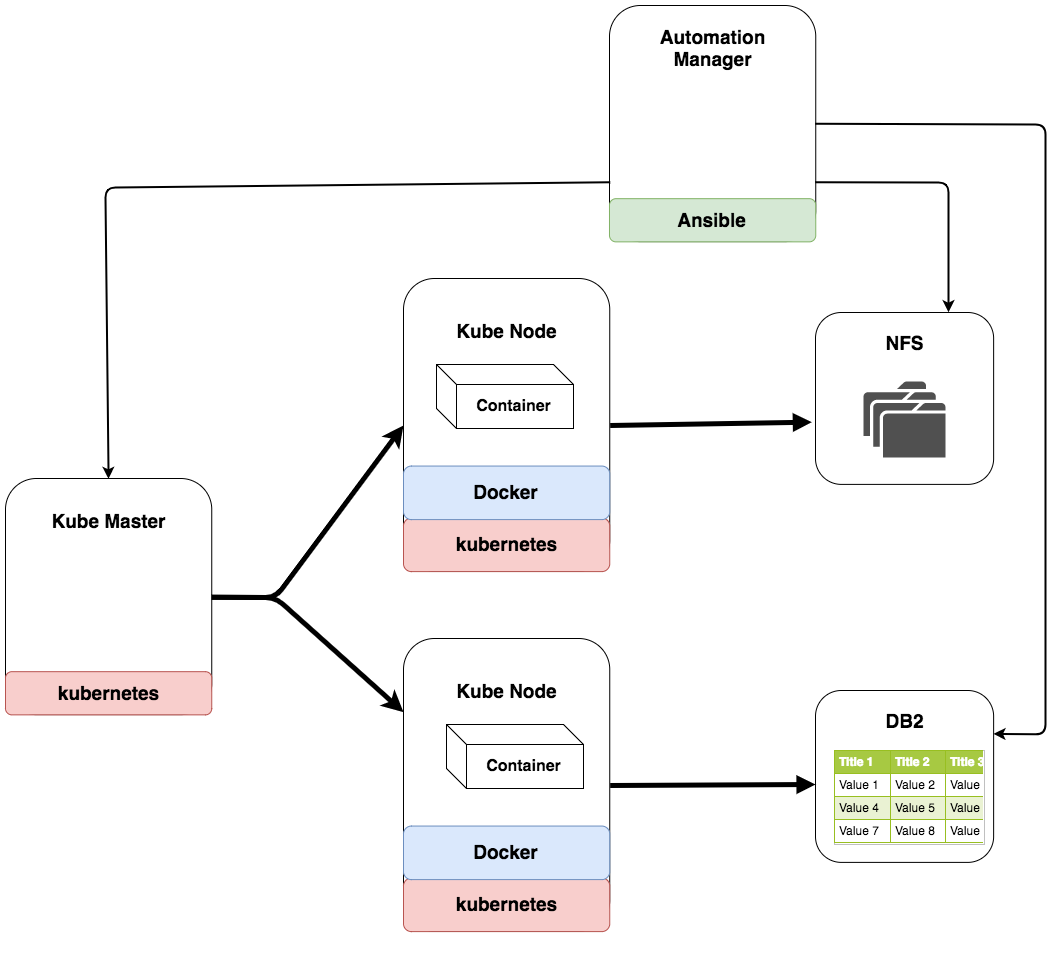
\includegraphics[width=0.8\textwidth,keepaspectratio=true]{capitoli/imgs/EnvironmentsComponentDiagram.png}
	\caption{L'ambiente di sviluppo di BigFix SaaS}
	\label{ambs}
\end{figure}


\section{Re-working degli installer del server e del relay di BigFix}
Il server e il relay di BigFix hanno i loro tradizionali installer relativi alla versione on premise del prodotto. Ovviamente è stato necessario un grosso lavoro di re-working di questi componenti per fare in modo che risultassero molto più leggeri e adatti al deployment in un container.

\section{Le immagini Docker}
Docker consente di deployare i container partendo da immagini di una repository fornita da Docker stesso. Nel nostro caso si è scelto di porre come base di tutti i container del servizio una macchina Linux CentOS 7 sia per i relay che per i server, una scelta dettata da esigenze aziendali. Docker fornisce delle versioni a container di molti sistemi operativi in modo da personalizzare secondo le proprie esigenze i container che si vanno ad implementare.

\paragraph{}
Questa macchina CentOS è ovviamente una versione molto embrionale dei servizi necessari per il prodotto. E' stato necessario creare delle directory di BigFix apposite per ospitare l'installer del server o del relay, a seconda dei casi. Si sono poste poi, all'interno di opportune cartelle, due file bash fondamentali per il deployment: install.sh e start.sh. Nella prossima sezione spieghiamo il loro compito.

\section{Docker containers, Pods e services}
I file bash di cui abbiamo parlato nella sezione precedente vengono in realtà eseguiti in contesti differenti. Install.sh viene chiamato in causa da Docker che in questo modo installa appunto il container. Successivamente Kubernetes chiama start.sh e avvia a tutti gli effetti i servizi di server e relay.
\paragraph{}
Ora occorre porre l'accento su come i container interagiscono con Kubernetes. La scelta in questo progetto è stata quella di avere una corrispondenza biunivoca tra i container di Docker e i pod di Kubernetes in modo da avere una semplicità di gestione dei container stessi. Vi è inoltre un ulteriore livello di astrazione sopra i Pod. Kubernetes offre infatti la possibilità di utilizzare il componente Service, che raggruppa in se uno o più pod. In questo progetto è stato utilizzato con il fine di poter utilizzare il pod nella rete in maniera più efficiente.
\paragraph{Yaml} 
I pod di Kubernetes utilizzano un particolare linguaggio di serializzazione lo YAML (YAML Ain't Markup Language). Esso è per certi versi molto simile all'XML e al JSON, ma è molto più essenziale e quasi tutto il suo contenuto rappresenta il dato da serializzare. I suoi punti di forza sono la manutenibilità e la flessibilità. Un file JSON infatti è anche un file YAML valido. All'interno dei file YAML si sono configurati tutti gli aspetti dei pod che sono necessari a Kubernetes per far partire i servizi relay e server con la struttura desiderata. Vediamo nella figura \ref{fig:yaml} un esempio di configurazione per un pod.
\begin{figure}
	\centering
	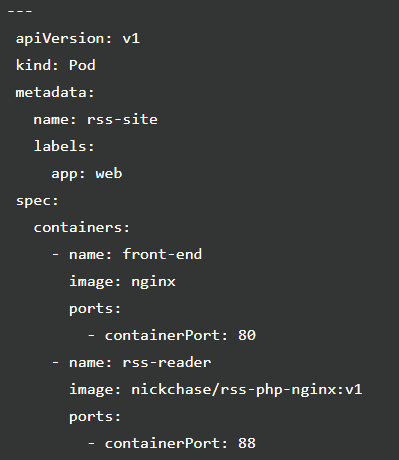
\includegraphics[width=0.5\linewidth]{capitoli/imgs/yaml}
	\caption{Esempio di YAML di configurazione per Kubernetes}
	\label{fig:yaml}
\end{figure}


\section{Modifiche al relay necessarie per la versione SaaS}
Il componente relay ha avuto bisogno di numerosi accorgimenti per permettere il suo funzionamento in prospettiva SaaS. Per sua natura, ha bisogno di numerose informazioni a riguardo del server al quale fanno riferimento. Per configurare il relay correttamente è necessario far rinvenire al relay alcuni file contenenti queste informazioni. Questa era una procedura che nella versione on premise veniva fatta a mano. Ora, nella realizzazione del servizio in SaaS, si è implementato un procedimento automatico che fa affidamento sullo storage condiviso fornito dall'NFS.
\paragraph{Relay scaling}
Altra proprietà del relay è la capacità di scalare adeguatamente rispondendo alle necessità. Durante il tipico utilizzo del prodotto è molto comune che il numero dei client o la mole di lavoro richiesta cambino dinamicamente. Superata una certa soglia di workload o un certo numero di client (circa 1000), un singolo relay non è più in grado di far fronte alle richieste, ma ha bisogno che parte dell'onere di lavoro venga presa in carico da una sua copia identica. Questo processo viene chiamato di "scale up". Analogamente possono verificarsi delle situazioni in cui le risorse allocate siano sovradimensionate rispetto al carico di lavoro. Fortunatamente Kubernetes fornisce un comando ad hoc per queste necessità. Questo strumento utilizza dei volumi condivisi di appoggio per fare si che le nuove copie dei relay non si debbano configurare da capo. Il nuovo relay infatti eredita dal primo sia tutte le configurazioni di BigFix e di Docker, ma anche la cache dell'altro relay, in maniera tale da essere subito operativo in pochi secondi. 
\paragraph{Air-gap}
Un'altro elemento che è necessario per abbattere i tempi per ottenere il nuovo relay funzionante è l'Air-gap. Senza scendere il dettagli e tecnicismi, questo componente ci consente di scaricare fixlet e altre configurazioni proprie di BigFix sul nuovo relay in tempi estremamente rapidi. 
\section{Automazione del Deployment}
Facciamo il punto della situazione cercando di individuare gli elementi che sono stati definiti fino a questo punto. Abbiamo da un lato la possibilità di deployare dei container che svolgano le funzioni di server o di relay perfettamente funzionanti, da un'altro c'è il database DB2 pronto a fornire persistenza a tutti i dati del cliente, da un'altro ancora altri componenti necessari all'ambiente per il corretto funzionamento, come l'NFS. Supponiamo che in un istante non predicibile un nuovo cliente acquisti la licenza ad utilizzare BigFix SaaS e abbia appena compilato la form con tutti i dati necessari. Cosa manca? 
\paragraph{}
Non è certo pensabile che a questo punto ci sia bisogno di un intervento umano per mettere a disposizione del nuovo cliente tutte le risorse necessarie. Ci si aspetta che il servizio sia disponibile nel giro di poche ore e la richiesta può essere avvenuta da qualunque parte del mondo e in qualunque momento della giornata.
\paragraph{}
Ecco quindi che è stato necessario un processo di software automation. Un processo automatico cioè che porti il prodotto ad essere pronto all'utilizzo da parte del nuovo cliente. Questo processo deve essere tollerante a malfunzionamenti e deve poter interagire con tutte le componenti facenti parte del sistema. Deve, in sostanza, comportarsi come una figura umana dedita all'istallazione. 

\subsection{Bash Scripting}
Nel progetto si è fatto largo uso del linguaggio Bash. Dovendo interagire con sistemi UNIX esso è stato spesso inserito in processi di automazione presenti negli scenari di gestione del sistema.
\paragraph{}
Bash, acronimo che sta per Bourne-Again-Shell, è un'interfaccia a riga di comando pensata per gestire i sistemi operativi UNIX nata alla fine degli anni '80. Come altri strumenti analoghi, oltre alla modalità interattiva, prevede anche la possibilità di creare script, con funzioni, cicli e costrutti tipici, e di eseguirli poi in blocco. Questi script sono contraddistinti dall'estensione .sh e dall'incipit "\#!/bin/bash", il quale indica il percorso della shell che dovrà eseguire lo script, Bash per l'appunto. 
\paragraph{Utilizzo degli script Bash nel progetto}
Gli script Bash sono stati di fondamentale importanza per il progetto. Data la loro versatilità e potenza è stato possibile utilizzarli per molti scopi di configurazione. Sono entrati, ad esempio, in dei flussi Ansible e Jenkins. Questi script venivano mandati tramite scp su opportune macchine e, una volta configurati i permessi, venivano eseguiti per svolgere i più disparati compiti necessari.
\subsection{Jenkins}
Il solo utilizzo di script bash non può garantire la corretta gestione di un'architettura così complessa come quella del SaaS di BigFix. Gli step di configurazione necessari ogni qualvolta si debba effettuare l'onboarding di un nuovo cliente sono numerosi e ripetitivi e quindi risulta molto utile adoperare un tool di automation.
\paragraph{}
Per questo motivo, almeno in un primo momento, si è utilizzato uno dei più diffusi strumenti di continuous integration: Jenkins. Esso è un progetto open-source nato da Oracle negli ultimi anni. Jenkins ci consente di eseguire e monitorare sistematicamente task ripetitivi come possono essere ad esempio i processi di building. Il sistema, disponibile tramite server web, ha la possibilità di essere integrato con innumerevoli plugin che lo rendono adatto a automatizzare i task più disparati sulle macchine più eterogenee. 
\paragraph{}
Nel lavoro di tesi si sono utilizzati proprio alcuni di questi plugin per permettere, a partire dalla macchina di Automation Manager in cui è installato, di orchestrare tutti i task sulle singole macchine dell'ambiente tramite ssh e scp.
\paragraph{}
Uno step preliminare che è stato necessario è quello di distribuire opportuni certificati alle macchine in modo da poter consentire la comunicazione tramite Jenkins. In questo modo non era più necessario esplicitare ogni volta la chiave ssh, ma si instaura una comunicazione a chiave pubblica e chiave privata. 
\paragraph{}
A questo punto necessario scrivere opportuni script bash per i diversi task che erano necessari per allocare le opportune risorse a ogni cliente.I tipici step necessari nelle diverse macchine del nostro ambiente sono i seguenti:
\begin{itemize}
	\item Creazione di opportune directory nell'nfs per ospitare file di configurazione.
	\item Validazione della licenza di utilizzo del servizio 
	\item Creazione e connessione al database per i dati dell'utente e configurazione dello stesso.
	\item Personalizzazione degli YAML relativi al server e al relay
	\item Creazione e avvio dei servizi del server
	\item Creazione e avvio dei servizi dei relay
\end{itemize}
\paragraph{}
Ovviamente per eseguire questi passaggi è necessario interagire con tutte le macchine dell'ambiente. Jenkins ha la responsabilità di guidare tutti questi passaggi e prendere opportune contromisure a eventuali malfunzionamenti. 
\begin{figure}[h]
	\centering
	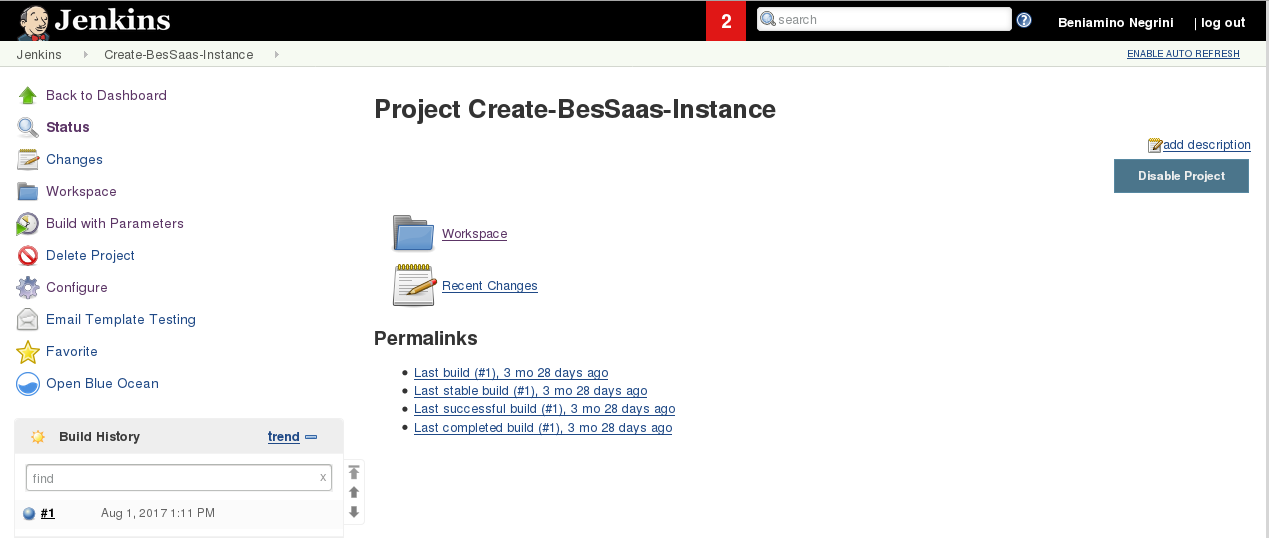
\includegraphics[width=0.7\linewidth]{capitoli/imgs/jenkisProj}
	\caption{Una delle schermate di configurazione di Jenkins}
	\label{fig:jenkisproj}
\end{figure}

\subsection{Ansible}
\paragraph{}
Dopo un confronto con il security operations team però, si è deciso di sostituire l'utilizzo di Jenkins con l'adozione di Ansible e UrbanCode Deploy. Il security operation è un team di IBM, situato in Irlanda, che avrà il compito di porsi tra i clienti BigFix SaaS e il team di sviluppo. Tra i suoi compito ci sono quello di monitorare le attività del SaaS, di porre rimedi a eventuali miglioramenti, di intervenire in caso di cali di prestazioni e molto altro. Dal confronto tra questi due team si è evinta la necessità di allineare i tool di BigFix SaaS a quelli degli altri prodotti cloud di IBM, in particolar modo UrbanCode. Un'altra motivazione che ha spinto la scelta verso UrbanCode è la possibilità di fare code promotion tra più ambienti di sviluppo, come vedremo in seguito. 
\paragraph{}
Relativamente alle modalità di utilizzo che si sono fatte in questo progetto Ansible rappresenta un'alternativa all'utilizzo di Jenkins. Ansible è uno strumento di automation nato nel 2012. Il tool si basa su due tipi di componenti, le macchine controllori che fanno partire l'automation e i nodi che sono le macchine dove avvengono eseguiti i task. 
\paragraph{}
Nel progetto è stata sfruttata molto la modularità di Ansible che permettere di sfruttare le strutture dei playbook e dei roles. Sostanzialmente un role è una successione di determinati task che hanno un fine e un target comune. I playbook sono delle collezioni di roles, i quali vengono così assemblati a piacimento per ottenere le configurazioni desiderate, come nel caso dell'ambiente di BigFix SaaS. 
\subsection{UrbanCode Deploy e code promotion}
C'è ancora un tool che è necessario integrare per garantire continuous integration e continuous delivery. Teniamo per un attimo in mente gli ambienti di sviluppo di cui abbiamo parlato nella sezione 7.2. Sarebbe molto utile che, ogni qualvolta viene effettuata una modifica al codice, un processo automatico integri questa modifica sequenzialmente negli ambienti di development, pre-production e production. Il passaggio tra questi ambienti può essere automatizzato ponendo come condizione di promozione all'ambiente successivo opportuni test automatici. Questo processo è chiamato di code promotion. 
\paragraph{}
Il tool in questione è un prodotto di IBM chiamato UrbanCode Deploy. Esso consente di coordinare e automatizzare le implementazioni delle applicazioni, le configurazioni di middleware e le modifiche ai database in ambienti di produzione e di test on-premise o basati su cloud. Nel progetto di tesi UrbanCode monitora l'esito dei playbook di Ansible e, in base al loro esito, decreta se fare o meno code promotion.
\begin{figure}
	\centering
	
\includegraphics[width=0.7\linewidth]{capitoli/imgs/ucd}
	\caption{IBM UrbanCode Deploy}
	\label{fig:ucd}
\end{figure}

\section{Scenario di onboarding di un nuovo cliente}
Questo scenario è stato il uno di quelli che ha richiesto più attenzione. Dato il coinvolgimento di molte componenti del sistema è stato uno dei primissimi ad essere realizzato e testato. 
\begin{figure}
	\centering
	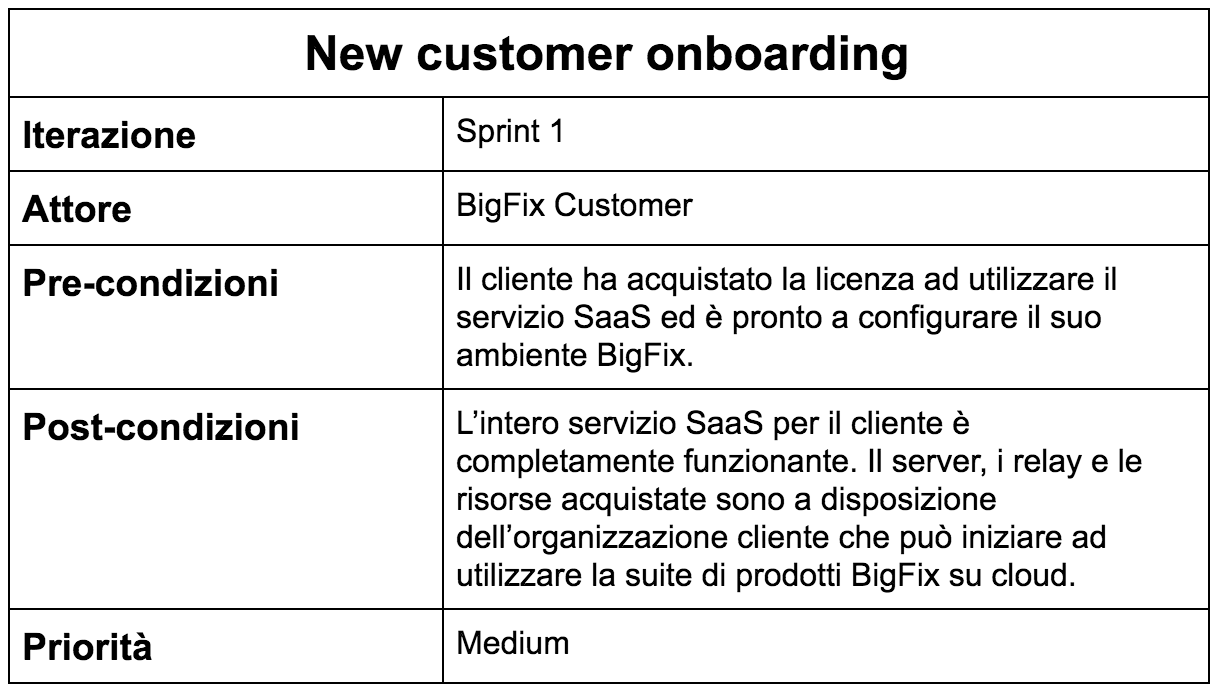
\includegraphics[width=0.7\linewidth]{capitoli/imgs/onbordingScenarioScheda}
	\caption{Scheda dello scenario di onboarding}
	\label{fig:onbordingscenarioscheda}
\end{figure}
\paragraph{}
L'utente, come primo step, riempie una form come quella nella figura \ref{fig:saasform} con tutti i dati necessari al sistema per configurare correttamente il suo ambiente. Tra questi dati necessario troviamo anche l'indirizzo email in modo da notificare la disponibilità del servizio al termine del processo. 
\begin{figure}
	\centering
	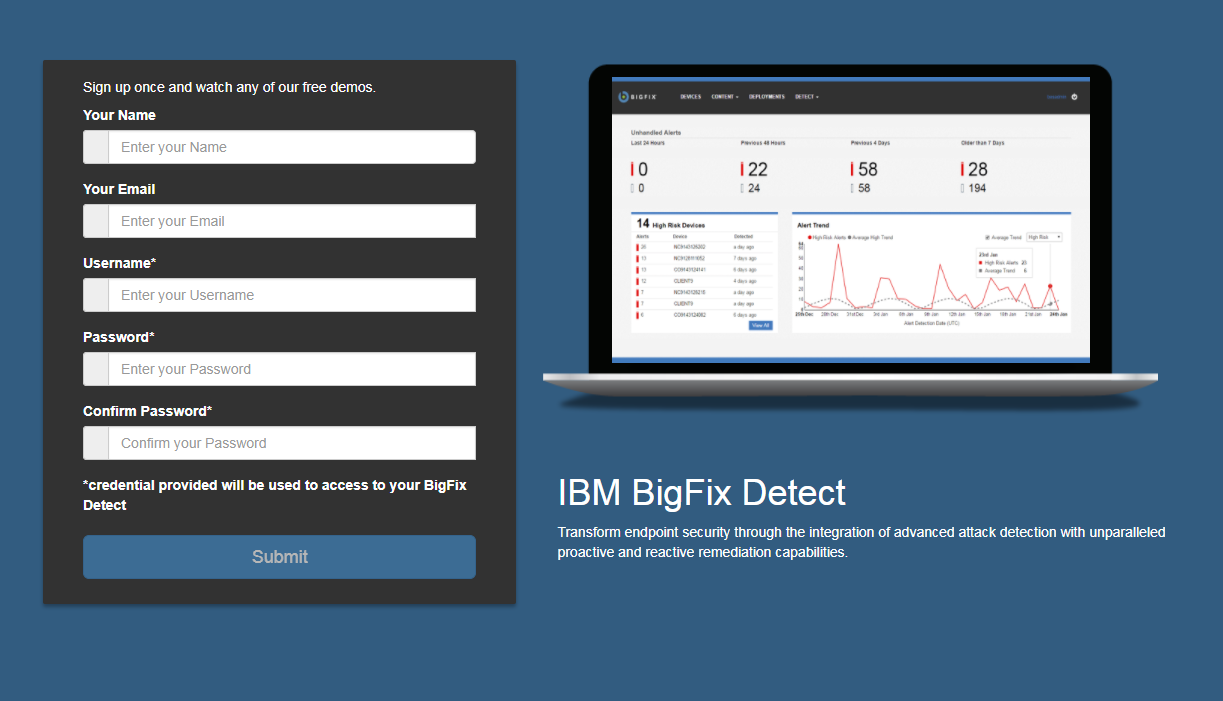
\includegraphics[width=0.7\linewidth]{capitoli/imgs/saasForm}
	\caption{Form per il cliente di BigFixSaaS}
	\label{fig:saasform}
\end{figure}
\paragraph{}
A questo punto entra in gioco l'automation di UrbanCode e Ansible che prende in pasto i dati appena inseriti nella from. Come prima cosa si mette in piedi il database per l'utente corrente. Questa operazione richiede un considerevole numero di configurazioni, che come anche le successive, vengono effettuate grazie a file bash opportunamente richiamati da Ansible. 
\paragraph{}
Una volta fatto partire il database, occorre "costruire" i file di YAML necessari per creare i pod di Kubernetes. Questi file vengono scritti partendo da un template che presenta dei placeholder. Questi placeholder rappresentano sia i dati dell'utente corrente, sia le versioni di build del prodotto stesso che, ovviamente, possono anch'esse variare. Il patching di questi file avviene tramite il linguaggio sed (stream editor), utilizzato per applicare espressioni regolari.
\paragraph{}
Gli YAML che ora sono personalizzati con i dati e le configurazioni del nuovo utente possono ora essere finalmente dati in pasto a Kubernets, il quale installa i container di Docker e avvia i servizi del server e del relay, come vediamo in figura. \ref{fig:kubedashboard}
\begin{figure}[h]
	\centering
	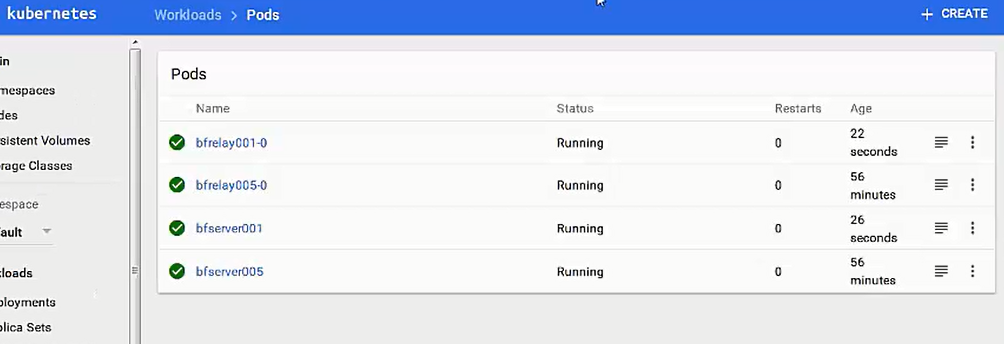
\includegraphics[width=0.7\linewidth]{capitoli/imgs/kubedashboard}
	\caption{Dashboard di Kubernetes}
	\label{fig:kubedashboard}
\end{figure}
\paragraph{}
Gli ultimi step da compiere sono quelli fornire un ip pubblico a questi servizi, in modo da renderli accessibili al cliente, e mandare una mail al cliente fornendo un comodo link per accedere ai servizi della suite BigFix SaaS. Come possiamo notare, dalla prospettiva dell'esperienza utente, è richiesto solamente che il cliente compili la form iniziale. Dopo una breve attesa i servizi sono pronti all'utilizzo direttamente dal dispositivo dal quale è stata compiuta la richiesta. Questo scenario può rappresentare una vera rivoluzione confrontandolo con l'analogo caso d'uso nella versione on premise di BigFix.
 

\section{Automazione del Testing}
Quella del test automation è un'attività molto importante nel contesto di un progetto SaaS. Non si può pensare infatti di fare continuous integration delle frequenti modifiche che si apportano ai microservizi effettuando un collaudo manuale del software. Occorre che un processo automatico si sostituisca all'uomo e effettui test approfonditi sia dal punto di vista sia funzionale che qualitativo, al termine dei quali si prendono provvedimenti o si portano le modifiche in produzione in modo che siano fruibili da tutti gli utenti. Il test non fa altro che comparare i risultati ottenuti dalle sue simulazioni con i risultati attesi dal prodotto. Al termine di ogni test è necessario che venga prodotto un report che possa essere consultabile dai team di operations. Alcuni progetti danno tanta importanza al test automation da sviluppare il realtà prima i test e poi il prodotto stesso. Si sviluppa poi il prodotto guidati dall'obiettivo di far superare tali test. Questa tecnica è chamata viluppo guidato dal test.
\paragraph{Continuous delivery}
In questo progetto si vuole che le modifiche che il team apporta al codice attraversiono un a serie di controlli prima di giungere alla totalità dei clienti. Le nuove modifiche infatti, entrano in un processo automatico composto di numerosi test. Dapprima vengono effettuati dei test funzionali, per appurare che le nuove modifiche non abbiano intaccato le funzionalità del prodoto, il nuovo codice guinge poi in un ambiente di Quality Assurance (QA) dove, sempre automaticamente vengono effettuati test di performance e di security a cascata. Se i nuovi componenti passano tutti i test previsti dal flusso automatico guingono finalmente in ambiente di produzione, ossia sono fruibili dai clienti. 
\paragraph{}
Anche questo ultimo passaggio, però, non è immediato. Sostituendo simultaneamente tutte le repliche del microservizio aggiornato si incorrerebbe in una non availability dell'intero sistema. Ciò non è accettabile in un servizio SaaS. Occorre aggiornare i container quindi un po' alla volta, redirigendo opportunamente il traffico su quei container ancora attivi o già aggiornati e riavviati. L'esperienza utente in questo modo non risentirà di nessun disservizio.
\subsection{Functional Test}
Come detto poc'anzi, i primi test in cui un nuovo microservizio deve fare i conti sono quelli funzionali. Presso IBM Security si sono canonizzati una collezione di test cases che verificano peculiaramente tutte le specifiche di BigFix nella sua versione onpremise. Questi test vengono svolti mediante un tool sviluppato nel team in cui lavorato che si basa su JUnit, un framework Java per compiere unit testing.
\subsubsection{JUnit}
JUnit è il più diffuso framework Java per compiere unit testing. Lo unit test rappresenta l'attività di testare singoli moduli software compiuta direttamente dagli stessi sviluppatori per testare singole porzioni di codice appena implementate. Lo scopo è quello di individuare eventuali bug da correggere prima di integrare le modifiche. JUnit consente di estendere le classi che intendiamo testare e tramite delle annotations indichiamo quali sono i metodi da invocare nei test cases.
\subsubsection{JUTAA}
JUTAA (Java Unified Test Automation Architecture) estende proprio JUnit. Presso IBM si è realizzato questo tool per migliorare la qualità dei test effettuati su BigFix e aumentarne il riuso. L'architettura è relativamente semplice. Una macchina funge da JUTAA master è può interagire sia con i server di BigFix che con i relay in modo da far girare su di essi i test case. Questi sono opportunamente raggruppati e catalogati. Per comunicare con le macchine slave JUTAA utilizza un'altro componente IBM, denominato STAF (Software Testing Automation Framework). Vediamo nella figura \ref{fig:jutaaarchitecture} una schematizzazione dell'architettura di JUTAA.
\begin{figure}[h]
	\centering
	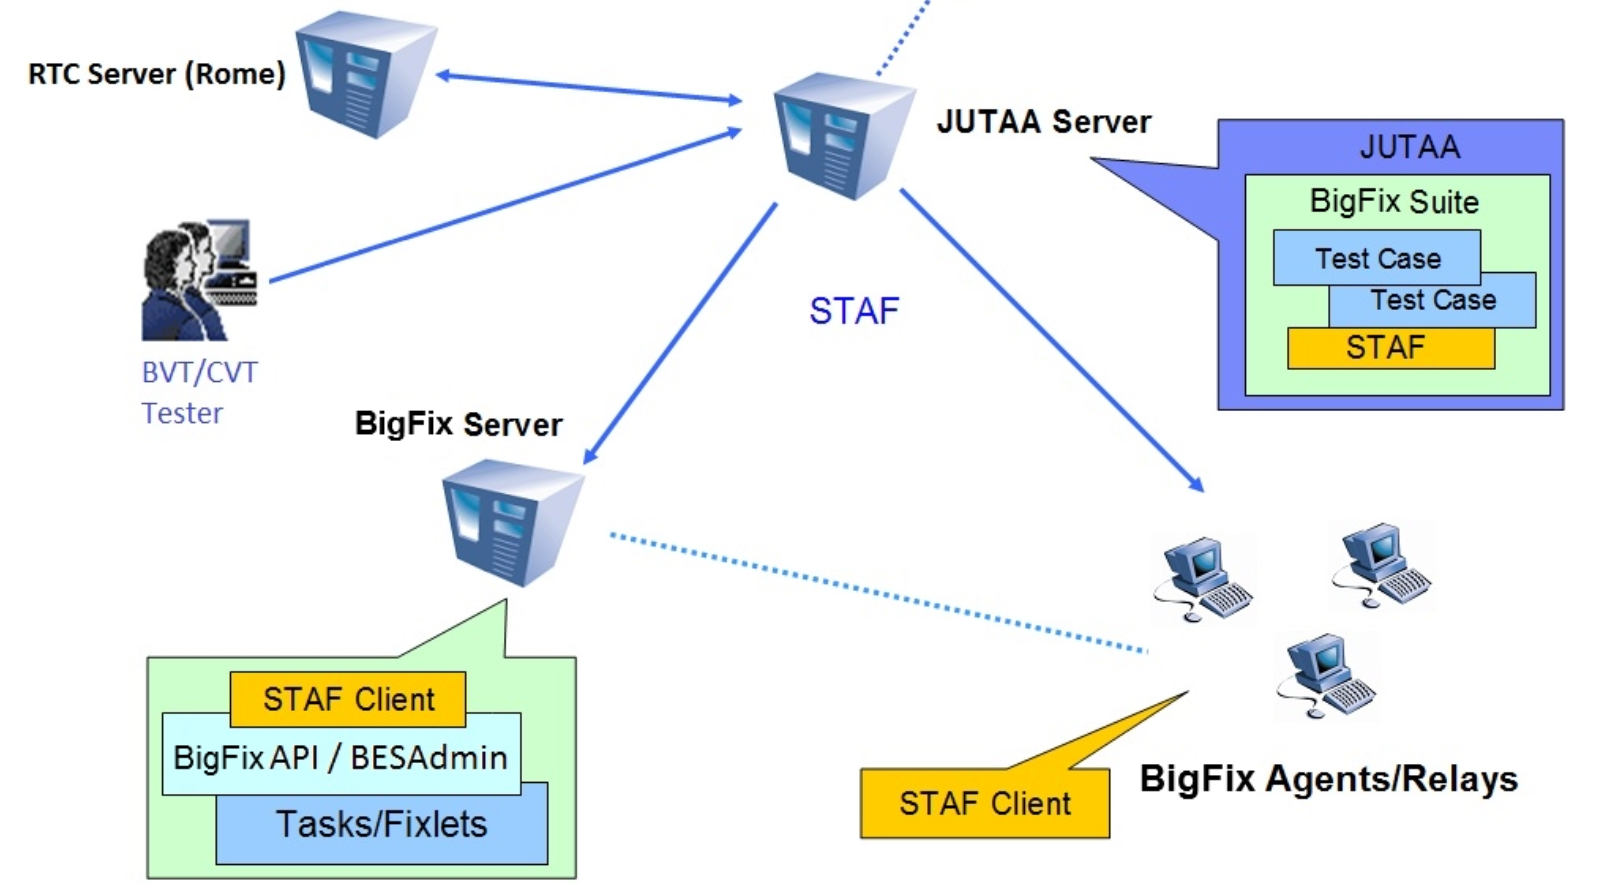
\includegraphics[width=0.7\linewidth]{capitoli/imgs/jutaaarchitecture}
	\caption{Architettura di JUTAA}
	\label{fig:jutaaarchitecture}
\end{figure}
\paragraph{Step per eseguire un test con JUTAA}
\begin{itemize}
	\item Test costruction \\
	JUTAA presenta una struttura modulare. E' possibile assemblare ad hoc i test di cui si ha bisogno tramite due file di configurazione in xml: env.xml e suite.xml. 
	\item Test execution\\
	Tramite un main.java viene lanciata la suite di test precedentemente dichiarata. Il framework scarica automaticamente il software più aggiornato da una repository.
	\item Test results analisys \\
	Tramite opportuni accorgimenti si raccolgono e si visualizzano i risultati dei test, determinando eventuali malfunzionamenti.
\end{itemize}
\subsection{Pre-production environment}
A questo punto il software è pronto per passare nell'ambiente di pre-production. Quì i servizi devono superare gli ultimi ostacoli, ossia i test qualitativi. In sequenza verranno effettuati test di security, di performance e di penetration al termine dei quali il prodotto entra in rolling release. Questo ambiente è curato dagli esperti di Quality Assurance che utilizzano metodi consolidati di testing come andremo a vedere nelle prossime sezioni.
\subsection{Security Test}
Una tematice di testing fondamentale per un servizio SaaS è quella di security. In questo ambito, per BigFix SaaS si compiono due tipi di indagini differenti. Una riguarda le exposure di sicurezza e una la riservatezza dei dati.
\subsubsection{Image Compliance}
Il concetto di base è che ogni componente o tecnologia che man mano si aggiunge al progetto ha delle vulnerabilità ben note. Il test si basa su una precisa descrizione e ctalogazione di queste vulnerabilità. All'aggiunta di un nuovo componente software, Image compliance va a controllare se questo componente potrebbe esporre il prodotto a qualche vulnerabilità. Nel caso affermativo si va a controllare se quela vulnerabilità è stata adeguatamente coperta in modo da renderne ilservizio immune. Questo compito è svolto da un tool di un progetto open source denominato clair.
\begin{figure}[h]
	\centering
	
\includegraphics[width=0.5\linewidth]{capitoli/imgs/clair}
	\caption{Clair}
	\label{fig:clair}
\end{figure}
\subsubsection{AppScan}
AppScan è un prodotto di IBM che ha come finalità quella di monitorare la vulnerabilità dei dati sensibili. Nel caso specifico di BigFix occorre porre molta attenzione a questa tematica in quanto i dati delle singole aziende clienti sono molto sensibili e la filosofia del multitenancy espone a notevoli rischi. 
\begin{figure}[h]
	\centering
	
\includegraphics[width=0.5\linewidth]{capitoli/imgs/ibm-appscan-logo}
	\caption{IBM AppScan}
	\label{fig:ibm-appscan-logo}
\end{figure}

\subsection{Performance Test}
I test di performance devono stabilire se il prodotto è conforme a dei parametri che sono stati definiti in fase di progettazione. Per fare ciò si sono implementati in IBM Security dei simulatori che, mediante l'utilizzo di hardware molto potente, riesce a simulare l'utilizzo del prodotto con un carico di lavoro considerevole. Questi simulatori sfruttano diverse tecnologie per rendere la simulazione più fedele possibile ad un utilizzo reale.

\subsection{Penetration Test}
Il penetration test per il prodotto BigFix SaaS è ancora in fase di studio. Questi tipi di test sono quelli relativamente più complessi in quanto si basano sulla simulazione di attacchi da parte di utenti malintenzioanti. E' in corso una fase di studio nell'individuazione di tecniche e tool di automation di questi tipi di test che, se volgliamo, possono essere i più ardui da automatizzare in quanto si basano su comportamenti umani meno prevedibili rispetto alle dinamiche delle altre tipogie di test.

\subsection{Rielaborazione degli output del testing}
Gli output di questa grande mole di test occorre che siano approfonditamente analizzati e interpretati per decretare se una nuova modifica del prodotto che si esegue nei continui cicli di produzione possa essere distribuita presso i clienti. Per questo è necessario svilupare un componente che sia in grado di prendere decisioni riguardo al passaggio tra i diversi ambienti di produzione del prodotto e possa presentare i risultati rielaborati al personale incaricato.

\section{Scenario di upgrade del servizio}
Questo scenario vede come attori del sistema il team di DevOps. E' anche questo uno scenario emblematico del passaggio al SaaS in quanto mostra le peculiarità di un aggiornamento del prodotto, o per meglio dire una parte di esso, ovvero i microservizi.
\begin{figure}[h]
	\centering
	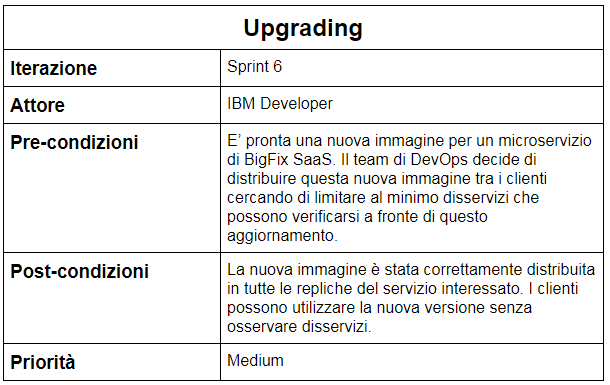
\includegraphics[width=0.7\linewidth]{capitoli/imgs/upgradescenarioScheda}
	\caption{Scheda dello scenario di onboarding}
	\label{fig:upgradescenarioscheda}
\end{figure}
\paragraph{}
La problematica principale da risolvere è quella mantenera un'alta availability del sistema nonostate alcune sue componenti vengano aggiornate e sostituite. Prima di giungere ai clienti però, 

\section{Il passaggio all'ambiente di produzione}
kubernetes -> ip pubblico, dns
portare questo sezione nel deployment



  \chapter{Conclusioni}

Questo lavoro di tesi ha visto la realizzazione, nel corso dei mesi, di un Software as a Service per l'azienda IBM. Una suite di servizi su cloud che permettesse di rivoluzionare i tool di IBM facenti parte della famiglia BigFix, una serie di prodotti per la security aziendale. Questi strumenti erano accessibili solamente nella tradizionale versione on premise. Il cliente doveva avere cioè a disposizione una infrastruttura notevole per poter permettere a BigFix di svolgere le proprie mansioni. Questo relegava il prodotto solo a clienti di grandi dimensioni che potevano permettersi ciò. 
\paragraph{}
Con la versione cloud di IBM BigFix, invece, l'unico componente che deve risiedere fisicamente presso il cliente è un agent installato su ogni endpoint fisico da controllare. Tutta la logica di controllo e le infrastrutture necessarie sono trasferite presso il provider del servizio cloud, ovvero IBM stessa.

\paragraph{}
Per adottare questa nuova filosofia è stato necessario riprogettare completamente il prodotto. Il lavoro è stato caratterizzato da una corposa fase di design, coinvolgendo molti stackeholders e potenziali clienti, ma anche personale di IBM come sviluppatori e futuri addetti all'assistenza. Adottando framework di progettazione e sviluppo come il "Design Thinking" e lo SCRUM, con un processo agile iterativo e incrementale, si è definita un'architettura dall'alto livello qualitativo e si è realizzato un prototipo di prodotto pronto per essere sperimentato e messo poi sul mercato.
\paragraph{}
Si è scomposto il prodotto con un'architettura a microservizi e si sono utilizzate le più affermate tecnologie cloud come Docker e Kubernetes. E' stato fondamentale, in tal senso, adottare l'utilizzo di software container per rendere indipendenti i singoli servizi. In una seconda fase poi è stato necessario orchestrare tutte le componenti contestualizzandole in pratiche di DevOps e continuous integration.

\section{Sviluppi futuri}
Il prodotto realizzato in azienda è, come detto prima, un prototipo. Questo verrà attentamente analizzato, presentato a potenziali clienti e valutato. Se l'azienda lo riterrà opportuno, verrà finalmente, dopo opportuni adattamenti, inserito nel catalogo e commercializzato. Occorrerà certamente raffinarne ulteriormente l'architettura a microservizi tenendo ben presente la divisione delle responsabilità per ognuno di essi. Una volta giunti a regime di produzione, si potranno aggiungere liberamente nuovi servizi a seconda delle necessità.
\paragraph{}
Un altro importante aspetto è perseverare sulla via della continuous delivery e della continuous integration. Queste pratiche faranno apprezzare maggiormente il loro contributo quando il prodotto verrà messo sul mercato. A quel punto i sempre più continui feedback degli utenti porteranno a un progressivo e definitivo miglioramento del servizio stesso.
\paragraph{}
Dal punto di vista delle tecnologie utilizzate, un'altra opportunità sulla quale si sta riflettendo è quella di adottare un database cloud nativo fornito da IBM Cloud. Questa scelta marcherebbe una forte differenza con le tradizionali architetture database e consentirebbe di integrare anche la persistenza in uno scenario di architettura cloud a microservizi.
\paragraph{}
Un prodotto di questo tipo, con il suo particolare mercato, è ovviamente soggetto a tante possibili future evoluzioni. I feedback e i futuri utilizzi del sistema porteranno continuamente maggior conoscenza e consentiranno al prodotto di essere sempre più al passo con le esigenze degli utenti.

\section{Considerazioni}
La realizzazione di questo servizio è stato un progetto molto sfidante e impegnativo, ma al tempo stesso mi ha visto affiancato da un team molto esperto e competente. Per questo è doveroso ringraziare tutto il team IBM di BigFix e in particolar modo l'ing. Bernardo Pastorelli per la sua disponibilità unita alla grande competenza. 
\paragraph{}
Il bagaglio di conoscenze acquisito durante questi mesi di lavoro è notevole sia sotto l'aspetto tecnico che dal punto di vista di gestione del ciclo di vita dei progetti. Al termine di questa importante esperienza è stato molto gratificante vedere apprezzato il lavoro di team in ambito dirigenziale aziendale sia a livello nazionale che internazionale. Ma soprattutto è stato ancora più appagante vedere come l'esperienza personale di tirocinio in IBM sia stata apprezzata e giudicata positivamente nella sede in cui si è lavorato.

\paragraph{}
Da un punto di vista tecnico, il prototipo si presenta già in uno stato molto avanzato. E' necessaria, a questo punto, solamente un'attenta indagine comprendendo se sono necessarie ulteriori modifiche al prodotto per renderlo definitamente pronto al suo utilizzo a livello industriale.
\paragraph{}
La strada intrapresa è sicuramente quella giusta. Il cloud computing rappresenta uno dei pilastri del futuro del software e orientarsi verso queste tecnologie significa aprirsi a nuovi scenari di utilizzo e a sempre più nuove opportunità. Non è fantascientifico immaginare che in un futuro molto prossimo ci si concerti solamente verso un utilizzo del software come servizio. Potrebbe non avere più senso detenere software e risorse localmente, ma ciò che farà la differenza sarà la fruizione delle risorse e dei prodotti. Ad esempio ci si potrebbe non preoccupare più di acquistare un personal computer con elevate specifiche hardware; basterà un prodotto che possa garantire un adeguato interfacciamento con risorse distribuite allocate dinamicamente. Risorse che in questo modo possono essere molto più prestanti e tecnologicamente avanzate.
\paragraph{}
In generale, in un mondo sempre più consumistico, in cui la maggior parte delle ricchezze sono sprecate, il cambio di prospettiva verso un utilizzo sapiente delle stesse e verso una sorta di "multi-tenancy" delle risorse comuni, può rappresentare una svolta considerevole.
  \chapter{Ringraziamenti}

«Come facciamo a scoprire qual è la nostra missione?
Scalate la montagna che avete di fronte, attraversate il fiume davanti a voi.
Non possiamo sapere quale montagna scaleremo in futuro fino a quando non avremo superato quella che abbiamo di fronte.
Anche se questa	scelta vi fa soffrire, anche se non ne avete voglia o avete timore di ciò che possono pensare gli altri, scalate la montagna davanti a voi senza fuggire;
allora la vostra visuale si amplierà sempre di più.
Riuscirete a vedere molto lontano e capirete chiaramente la strada giusta da percorrere.
La distanza tra zero e uno è molto più grande di quella tra uno e cento.
Anche un viaggio di mille miglia inizia sempre da un primo passo».

\paragraph{}
Qualche anno fa mi è capitato di leggere questo discorso quando era il momento di scegliere quali fossero i primi passi da compiere. Ora che è terminato solo il primo dei sentieri, ripenso alla strada percorsa e mi rendo conto che non sono mai stato solo.

\paragraph{}
Ringrazio i miei nonni che mi hanno accompagnato già dai primissimi metri, che hanno trasmesso le mie radici e accompagnato nel mio futuro.

\paragraph{}
In ogni ostacolo che ho incontrato davanti a me ci sono stati sempre i miei genitori ad affiancarmi per superare ogni difficoltà, a incoraggiarmi e supportarmi facendo sacrifici per non farmi mancare mai nulla. In questo percorso si è unita presto a noi una piccola peste, portando un'allegra confusione... grazie sora!

\paragraph{}
Un grande ringraziamento va anche ai miei amici, con i quali ne abbiamo passate tante, ma alla fine siamo sempre tornati a casa sani e salvi (più o meno), come se non fosse successo niente.

\paragraph{}
La strada mi ha portato a proseguire il mio percorso in questa università. Indubbiamente sono stati cinque anni formanti ma soprattutto tra i più divertenti! Dalla MyShop Srl con la quale conquisteremo il mondo agli approcci aggggili dei tre profeti e bulli vari... non ho trovato dei semplici colleghi di corso, ma una classe affiatata, con la quale svolgere i progetti è un vero divertimento. Non posso inoltre non ringraziare amici e professori che mi hanno accolto a Dublino, in una esperienza breve ma ricca di avventure e soddisfazioni.

\paragraph{}
In particolar modo un ringraziamento particolare va al professor Cicerone per avermi accompagnato in tutto il percorso universitario facendomi appassionare all'ingegneria del software e per avermi accolto come suo relatore.

\paragraph{}
Il lavoro svolto in questo progetto di tesi non sarebbe mai stato possibile senza l'opportunità che mi è stata concessa dal team di IBM BigFix di Roma. Ho avuto la possibilità di essere ospitato in una grande famiglia e per questo non posso non ringraziare Dante, Max e tutto il team di BigFix per il loro aiuto; Marco per essere stato un attentissimo tutor e Bernardo per avermi seguito con la sua eccezionale esperienza durante tutto lo stage.

\paragraph{}
Infine l’ultimo dei ringraziamenti, ma non per importanza, va a una persona che ha portato i colori sul mio sentiero da quando abbiamo iniziato a percorrerlo insieme. Una persona che mi ha dato forza per credere in me stesso incoraggiandomi a dare il meglio, che sopporto ogni giorno… ma sopratutto mi sopporta ogni giorno!

\paragraph{}
Strada da fare ce n'è ancora tanta, ma guardando a quella già fatta mi accorgo di non essere mai stato solo. Grazie a tutti voi!

\bibliografia{bibliografia/bibliografia}{}

\appendice
  \printglossary
  \chapter{Tecnologie Utilizzate(template di prova - ANCORA DA SCRIVERE)}
  \section{Linguaggi di programmazione}
    \begin{itemize}
     \item PHP 5.4.7 \\
     \href{http://www.php.net/}{http://www.php.net/};
     \item Javascript \\
     \href{http://www.w3.org/standards/webdesign/script}{http://www.w3.org/standards/webdesign/script};
    \end{itemize}
   \section{Linguaggi di Markup e Stile}
    \begin{itemize}
     \item HTML4/HTML5;
     \item CSS/CSS3;
    \end{itemize}
   \section{Framework}
    \begin{itemize}
     \item Smarty Template Engine \\
	\href{http://www.smarty.net/}{http://www.smarty.net/};
     \item JQuery\\
	\href{http://jquery.com/}{http://jquery.com/};
     \item JQueryUI\\
	\href{http://jqueryui.com/}{http://jqueryui.com/};
     \item beContent\\
	\href{http://www.becontent.org/}{http://www.becontent.org/};
    \end{itemize}
   \section{Ambiente di Sviluppo}
    \subsection{Eclipse}
      Per Eclipse sono state utilizzate due versioni differenti, la 4.2.2 in ambiente Windows e la 3.8.0 in ambiente Ubuntu/Linux \\
      \href{http://www.eclipse.org/}{http://www.eclipse.org/} \\
      Inoltre è stato utilizzato il pacchetto
      \begin{itemize}
       \item PHP Development Tools 3.1.1 \\
       \href{http://projects.eclipse.org/projects/tools.pdt}{http://projects.eclipse.org/projects/tools.pdt};
       
      \end{itemize}
    \subsection{Piattaforma Web}
      \subsubsection{XAMPP}
      \href{http://www.apachefriends.org}{http://www.apachefriends.org}
      \begin{itemize}
       \item Apache Web Server ver. 2.4.3 \\
	  \href{http://httpd.apache.org/}{http://httpd.apache.org/};
       \item MySql Database Management System ver. 5.5.27 \\
	  \href{http://dev.mysql.com/}{http://dev.mysql.com/};
      \end{itemize}
    \subsection{Browser Testing}
      \subsubsection{Mozilla Firefox}
	\begin{itemize}
	 \item Firebug ver 1.11.2 \\
	  \href{http://getfirebug.com/}{http://getfirebug.com/}
	    \begin{itemize}
	     \item Plug-In Validator ver. 0.0.6 \\
	      \href{https://addons.mozilla.org/it/firefox/addon/validator/}{https://addons.mozilla.org/it/firefox/addon/validator/};
	     \item Plug-In Google Page Speed ver. 2.0.2.3 \\
	      \href{https://developers.google.com/speed/pagespeed/?hl=it-IT}{https://developers.google.com/speed/pagespeed/?hl=it-IT};
	    \end{itemize}
	\end{itemize}
      \subsubsection{Google Chrome}
	\begin{itemize}
	 \item Strumenti per gli sviluppatori integrati 
	\end{itemize}
      \subsubsection{Responsive Testing}
	\begin{itemize}
	 \item Viewport Resizer- Responsive Design Bookmarklet \\
	 \href{http://lab.maltewassermann.com/viewport-resizer/}{http://lab.maltewassermann.com/viewport-resizer/} ;
	\end{itemize}




  


  
\begin{dedication}
  
\end{dedication}
\begin{dedication}
  \textit{Dedica a fine pagina}
\end{dedication}

\end{document}

%%%%%%%%%%%%%%%%%%%%%%%%%%%%%%%%%%%%%%%%%%%%%%%%%%%%%%%%%%%%%%%%%%%%%%%%%%%%%%%%

